\documentclass[12pt]{article}

\usepackage[utf8]{inputenc}
\usepackage[T1]{fontenc}
\usepackage[portuguese]{babel}
\usepackage[top=2cm, bottom=2cm, left=2.5cm, right=2.5cm]{geometry}
\usepackage{graphicx}
\usepackage{listings}
\usepackage{indentfirst}
\usepackage{ucs}
\usepackage{amsmath}
\usepackage{amsfonts}
\usepackage{amssymb}
\usepackage{makeidx}
\usepackage{breqn} %necessario para usar o ambiente 'dmath'
\usepackage{multicol}
\usepackage{multirow}
\usepackage{rotating}
\usepackage{scalefnt}
\usepackage[footnotesize,bf]{caption} 

%--- pacote para figuras
\usepackage{epsf}
\usepackage[dvips]{epsfig,graphicx}
\usepackage{subfigure}
\usepackage{float}%Coloca a figura onde desejo

\title{Minimização de Criticalidades de Redes Elétricas com foco na qualidade da Estimação de Estado}
\author{Vinícius Biajoni Braga Flôr\\ Instituto de Computação UFF- Niterói- RJ- Brasil\\ Inteligência Computacional 2020.1}
\date{Professor: Luiz Satoru Ochi}


\begin{document}

\maketitle

%\doublespacing
\abstract{\textbf{A Estimação de Estado (EE) é uma etapa vital da operação em tempo real de um Sistema Elétrico de Potência. Para a garantia dessa estimação, uma alocação adequada das medições nessa rede é fundamental para garantir sua observabilidade com o mínimo de custo possível. Diversos trabalhos se empenharam na solução desse problema e a literatura apresenta um conteúdo vasto nessa vereda. Entretanto, para a garantia de uma EE de qualidade deve-se considerar a presença das criticalidades das medidas dessa rede, pois essas colocam em risco a observabilidade e a capacidade de detecção e identificação de dados espúrios. Com isso, a presente proposta visa resolver um problema combinatorial novo, o qual envolve a alocação ótima de lotes de unidades de medição com o objetivo de minimizar essas criticalidades, principalmente aquelas de cardinalidades inferiores. Para solução foram testadas duas metaheurísticas a primeira chamada de GRASP-VND e a segunda de VNS-VND. Para os testes foram utilizadas as redes IEEE 30 e 118 barras que são tradicionais na literatura relacionada.}}
%\begin{flushleft}
%\maketitle
%\title\textbf{Resumo} 
%\end{flushleft}


\section{Introdução}

Em redes elétricas existem diversas atividades que interagem entre si para garantir que a operação do sistema garanta uma boa confiabilidade. Uma função básica para essa operação é a chamada Estimação de Estado, a qual deve estimar com qualidade os valores das tensões e ângulos dos barramentos da rede. Isto posto, para se garantir a Estimação de Estado necessita-se que a rede seja observável \cite{Abur04}-\cite{Mont99}. Sendo assim, são necessárias algumas condições para se observar a rede, as quais envolvem características topológicas (conexões entre barras) e posicionamento das unidades de medição e suas respectivas medidas associadas.

Nos Sistemas Elétricos de Potência, uma informação fundamental é a topologia da rede. Essa indica as relações entre as barras da rede. Havendo essa informação, o problema para garantia da observabilidade da rede se torna inerente à alocação adequada das UMs(Unidades de Medição). Dessa forma, deseja-se uma alocação tal que minimize o custo de instalação porém ao mesmo tempo garanta que o estado da rede seja estimado. Esse problema apresenta uma natureza combinatorial e se agrava a cada restrição ou condição que seja inserida. Essa abordagem já foi amplamente explorada na literatura e existem muitos trabalhos que solucionaram esse problema de diversas maneiras.

Em relação à alocação de UMs diversos trabalhos já foram publicados, alguns com abordagens semelhantes outros com algumas variantes. Entretanto, o foco se manteve na alocação mínima de UMs para garantir a observabilidade da rede. Nesse contexto, basicamente, a literatura está dividida em trabalhos que envolvem técnicas determinísticas e outros que seguem a abordagem das metaheurísticas. Em \cite{Marin03} utilizou-se o conceito de Algoritmos Genéticos(AG) para a alocação ótima de UMs. Outro trabalho baseado em AG foi apresentado em \cite{Aminifar09} onde se utilizou um conceito de imunidade no algoritmo genético, entretanto esse trabalho apresentou sérios problemas em relação ao tempo de execução. Por fim, uma abordagem  envolvendo teoria de grafos e AG foi apresenta em \cite{Milosev03}, neste trabalho considerou-se a possibilidade de perdas de linhas de transmissão. Outras técnicas já foram abordadas na literatura, como Particle Swarm Optimization(PSO), conforme apresentado em \cite{PSO}. Em \cite{BPSO} os autores sugeriram uma forma alternativa do algoritmo anterior chamado de \textit{binary particle swarm optimization} (BPSO), o objetivo do trabalho era alocar as UMs para garantir a total observabilidade da rede e maximizar a redundância das medidas. Outras abordagens baseadas em Simulated Annealing,  Busca Tabu e busca em árvore já foram propostas, respectivamente em \cite{SA}, \cite{TS} e \cite{Tree}. Em relação a métodos exatos alguns foram explorados ao longo dos ano. A principal referência é o trabalho desenvolvido por Abur, em \cite{Abur04_opt}. Outros trabalhos com o uso de programação linear inteira foram abordados em \cite{Amin10},\cite{Gou08_1} e \cite{Gou08_2}. Outras abordagens e trabalhos poderiam ser listados, mas esses citados demonstram que o problema de alocação ótima de UMs para garantia de observabilidade já está bastante estabelecido. Uma revisão importante dos diversos trabalhos nesse contexto de observabilidade se encontra em \cite{ReviewAlloc}.

No presente trabalho uma nova abordagem é desenvolvida voltando-se o foco para a redução das criticalidades das medidas em uma rede observável. Para tal busca-se alocar da melhor maneira possível um lote pré-estabelecido de UMs. Esse processo envolve inúmeras combinações e torna-se complexo com o crescimento da rede e da relação entre barras disponíveis e tamanho do lote. De acordo com a revisão bibliográfica realizada, em relação aos trabalhos voltados a alocação para observabilidade, não foram encontradas na literatura propostas utilizando-se algoritmos como GRASP e VNS, os quais são amplamente conhecidos e aplicados em problemas da área de otimização combinatória. Essa ausência juntamente com a capacidade desses algoritmos lidarem com uma estratégia de busca-local para intensificação da solução mostra-se como uma vereda interessante para a exploração dessa nova abordagem, visto que a diferença entre uma alocação ótima e uma sub-ótima pode estar relacionada a uma única diferença entre barras com UMs alocadas. Assim sendo, adaptou-se as metaheurísticas GRASP e VNS para o problema em questão. Nas etapas de busca local utilizou-se a técnica VND com algumas estruturas de vizinhança. Por fim, para os testes utilizou-se as redes IEEE 30 e 118 barras apresentadas em trabalhos que envolvem identificação de criticalidades.

\section{Contextualização do Problema e Motivações}

Conforme apresentado nessa breve revisão, o problema de alocação ótima de UMs para observabilidade da rede é algo já bastante conhecido na literatura. Em contrapartida, muitas vezes se possui uma rede previamente planejada e já observável essa, porém, apresenta diversas características negativas que podem colocar em risco a qualidade e confiabilidade da operação do sistema elétrico. Uma dessas características são as chamadas criticalidades de medidas, as quais podem mascarar erros grosseiros em medidas e provocar problemas quanto à observabilidade da rede. Em um sistema elétrico essas criticalidades podem influenciar na qualidade da Estimação de Estado (EE) provendo resultados pouco confiáveis ao centro de operação. Em contrapartida a determinação de todas as criticalidades de uma rede é um problema de natureza combinatorial e bastante complexo, \cite{AbelTese16},\cite{Sou12} e \cite{BB16}. Devido a isso é possível estabelecer um grau de prioridade em relação às criticalidades de medidas que se deseja mitigar na rede. Essa escolha está relacionada tanto ao custo para a determinação das criticalidades de ordens mais superiores, quanto à questão de aplicabilidade prática visto que essas são as criticalidades que mais facilmente podem afetar a qualidade do processo de EE.

Para justificar a importância dessa análise pode-se recorrer à Figura \ref{fig1}. Observando-se essa tabela é possível extrair a importância associada a cada criticalidade da rede. Uma C1-tupla se refere a uma medida essencial à EE, ou seja, a ausência desta torna a rede não observável. Uma C2-tupla se refere a um par de medidas que estão associadas entre si, de forma que a perda de uma das medidas do par torna a restante uma medida crítica. É importante observar que apenas a indisponibilidade de ambas medidas torna a rede não observável. Já uma C3-tupla é um conjunto de três medidas correlacionadas as quais se perdidas em pares tornam a restante uma medida crítica. Essa lógica pode ser generalizada para k medidas conforme apresentado na Figura \ref{fig1}. Isto posto, a justificativa para a mitigação dessas criticalidades está relacionada ao processamento de erros grosseiros das medidas, no processo de EE. Conforme a Figura \ref{fig1}, um erro grosseiro em uma C1-tupla não pode ser detectado ou identificado. A presença de um erro grosseiro em uma das medidas de uma C2-tupla pode ser detectada, entretanto não se consegue identificar em qual das medidas esse erro se encontra. Por fim, em uma C3-tupla, os erros grosseiros simples podem ser detectados e identificados, porém se os erros foram múltiplos a identificação deixa de ser possível.

\begin{figure}[H]
	\centering 
	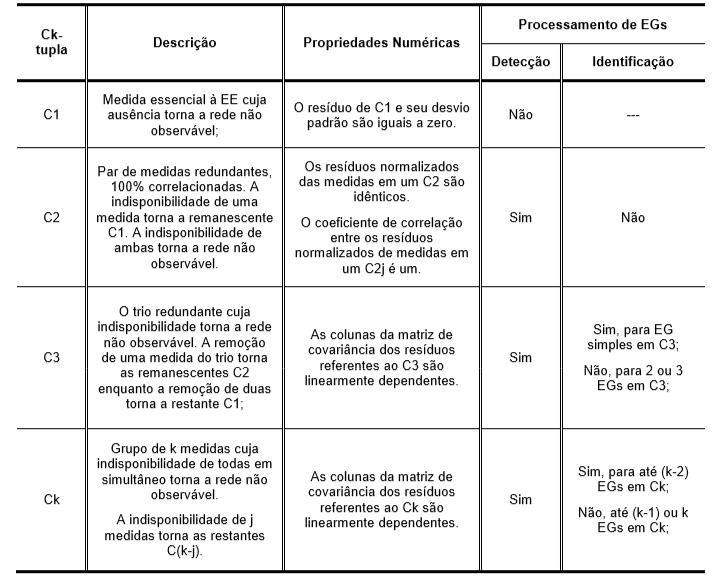
\includegraphics[scale=0.9]{figuras/Criticalidades-med.jpg}
	\caption{Relação entre criticalidades e capacidade de processamento de erros grosseiros.\cite{AbelTese16}}
	\label{fig1} % mudar a referencia de acordo com o desejado
\end{figure}

Com o conceito de criticalidades e a relação da vulnerabilidade do sistema de medição com as Ck-tuplas presentes, justifica-se o interesse em minimizar (ou mitigar) a presença desses conjuntos em uma rede. A ideia mais simples para solucionar o problema seria instalar o máximo possível de UMs nessa rede de maneira a mitigar grande parte das criticalidades de ordens inferiores. Entretanto, cada UM possui um elevado custo associado e, na prática, dispõe-se de pequenos lotes dessas UMs para serem dispostos a fim de mitigar essas criticalidade. Isto postp, o presente trabalho focará na instalação de pequenos lotes dessas unidades de medição, de forma a minimizar ao máximo as criticalidades de ordens inferiores.

O problema se baseia na redução das criticalidades de ordens inferiores através da alocação ótima de um lote UMs adicionai. Dessa forma, propõe-se uma nova abordagem em relação ao problema de alocação de UMs, o qual agora se baseia em uma estratégia de reforço da rede e de minimização das criticalidades. A consideração dessas é algo ainda não explorado nesses problemas e pode ser um campo fértil de novos trabalhos nesse sentido, principalmente pelo fato do elevado custo dessas UMs, resultando em lotes limitados e tornando o problema combinatorial. Essa complexidade eleva-se com o crescimento dos sistemas e da relação entre barras disponíveis para alocação e a dimensão de lotes de UMs para serem alocados. Devido a essa possibilidade de explosão combinatorial a utilização de um método de busca exaustiva pode ser impossibilitada. Assim sendo, a utilização de metaheurísticas se justifica e passa a ser uma forma factível para a obtenção de soluções de boa qualidade para qualquer instância avaliada.

\section{Estimação de Estado e Criticalidades de Medidas}

O processo de Estimação de Estado (EE) de um sistema elétrico de potência é considerado o pilar central das diversas funções do chamado sistema de gerenciamento de energia. Esse processo tem por objetivo prover dados confiáveis referentes às condições atuais de operação de uma rede elétrica \cite{Abur04}-\cite{Mont99}. A garantia de que a EE poderá ocorrer está contida no conceito de observabilidade. Uma rede é dita observável quando é possível, através de um conjunto redundante de medidas, obter-se todas as tensões complexas da rede. Na prática, cada barramento da rede pode ser entendido como um subestação de energia elétrica que funciona como ponto de conexão entre linhas de transmissão.Na sequência apresenta-se um breve resumo teórico para um entendimento básico das matrizes que envolvem o processo de EE e suas relações com a identificação das criticalidades de medidas.

O trabalho apresentado em \cite{Hand07} apresenta uma metodologia que permite avaliar essas criticalidades de maneira off-line, ou seja, previamente ao processo de EE. Para isso utiliza-se uma modelagem simplificada das matrizes associadas ao processo de EE tornando possível considerar apenas as medidas ativas da rede \cite{Abur04}, em outras palavras, apenas a componente real das medidas, desconsiderando as parcelas complexas. A matriz que associa os tipos de medidas com as barras as quais essas estão associadas chama-se matriz Jacobiana $\mathbf{H}$. Essa matriz é o cerne tanto do processo de estimação quanto do processo de identificação das criticalidades, isso porque as demais matrizes do problema são todas derivadas dessa matriz base. A Figura \ref{fig2} apresenta uma ilustração genérica de como se constrói uma matriz Jacobiana. As medidas convencionais são chamadas de fluxos e injeções ativas. Já as medidas fasoriais são referentes aos ângulos e fluxos ativos de corrente. Cada linha é referente a uma medida da rede e cada coluna está associada a uma variável de estado. Por fim, a variável $nb_i$, na Figura \ref{fig2}, indica o número de conexões que uma $i$ possui. No presente trabalho considera-se, por questão de escolha, apenas medidas convencionais providas pelas UMs. Entretanto, a consideração de medições fasoriais pode ser facilmente aplicada à modelagem.

\begin{figure}[H]
	\centering 
	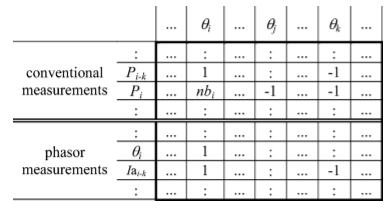
\includegraphics[scale=1.2]{figuras/Jacob.jpg}
	\caption{Matriz Jacobiana genérica.\cite{AbelTese16}}
	\label{fig2} % mudar a referencia de acordo com o desejado
\end{figure}

A partir da obtenção da matriz $\mathbf{H}$ pode-se derivar outra matriz importantíssima, chamada de matriz de ganho $\mathbf{G}$. Essa matriz é amplamente utilizada na literatura para determinar a capacidade de observar ou não uma rede. A presença de linhas linearmente dependentes indica a que a rede é não-observável \cite{Mont85} e \cite{AburObserv00}. A forma de obtenção da matriz de Ganho encontra-se na Equação \ref{eq1}, a qual depende basicamente da matriz Jacobiana e de uma $\mathbf{I}$ que na presente abordagem é uma matriz identidade. É importante salientar que no processo de EE a matriz $\mathbf{I}$ passa a ser chamada de $\mathbf{R}$ e  apresenta, em sua diagonal principal, a variância de cada medida.

\begin{equation}
	\mathbf{G= H^tR^{-1}H}
\label{eq1}
\end{equation}

O processo de determinação das criticalidades de medidas de uma rede não será discutido em profundidade no presente trabalho, porém maiores detalhes podem ser encontrados em \cite{AbelTese16} e \cite{BB16}. De maneira geral, a determinação das criticalidades de qualquer cardinalidade é um processo combinatorial e que depende da análise da matriz de covariância de resíduos $\mathbf{E}$. Essa é obtida a partir das matrizes $\mathbf{H}$ e $\mathbf{G}$ \cite{Quant13}, de acordo com a Equação \ref{eq2}.

\begin{equation}
	\mathbf{E= I - HG^{-1}H^t}
	\label{eq2}
\end{equation}

A matriz $\mathbf{E}$ é quadrada de ordem igual ao número de medidas do plano de medição. Assim sendo, para avaliar se um dado conjunto de medidas é uma Ck-tupla, constrói-se uma submatriz $\mathbf{E_a}$, a qual possui ordem k e envolve os elementos da matriz $\mathbf{E}$ que associam as medidas referentes a tupla em teste. Cada elemento de $\mathbf{E_a}$ pode ser obtido através das Equações \ref{eq3} e \ref{eq4}. Nessas $\mathbf{h_i}$ e $\mathbf{h_j}$ são vetores linha referentes às medidas i e j da matriz $\mathbf{E}$.

\begin{equation}
	\mathbf{E_a(i,j)= h_i(G)^{-1}h_ j^t}
	\label{eq3}
\end{equation}
	
\begin{equation}
	\mathbf{E_a(i,i)= 1 -  h_i(G)^{-1}h_ j^t}
	\label{eq4}
\end{equation}

Conforme dito, esse processo é combinatorial e apresenta elevado custo computacional conforme a cardinalidade k se eleva. Isto posto, o presente trabalho irá avaliar apenas tuplas críticas até a cardinalidade 3 visto que a busca por criticalidades muito elevadas seria pouco aplicável à pratica e muito custoso para estar inserido em um contexto de meta-heurísticas. Para a obtenção dessas criticalidades utilizou-se um algoritmo de força bruta (busca exaustiva) modificado, o qual utiliza o paralelismo de CPU para tornar o processo mais eficiente. Essa etapa é o cerne do cálculo da função objetivo (ou função de fitness) do processo de otimização, pois os resultados dessas criticalidades são utilizado para avaliar a qualidade de cada solução. Em trabalhos futuros o objetivo é tornar essa etapa mais otimizada utilizando-se outras abordagens, principalmente teoria de grafos.



\section{Alocação Ótima para Minimização de Criticalidades}

Em uma rede elétrica previamente planejada uma condição necessária para a realização da EE é a garantia da condição de observabilidade. Nesse sentido as UMs que se encontram previamente alocadas garantem essa condição. Em contrapartida, o conceito de observabilidade não é suficiente para garantir a robustez de uma rede em relação à qualidade do processamento de erros grosseiros da EE. Sendo assim, o reforço de um plano de medição considerando-se as criticalidades é uma forma de se melhorar esse quesito.

Uma rede com muitas criticalidades, principalmente de cardinalidades mais baixas, pode ser considerada de "pior" qualidade que outra rede também observável porém com criticalidades de ordens mais elevadas. Entretanto, essa análise não é direta e deve-se estabelecer um trade-off em relação a essas quantidades de criticalidades distribuídas por cada cardinalidade. Sendo assim, seja uma rede observável na qual se possui o conhecimento de um conjunto $\mathbf{C}$ de tuplas críticas. Deseja-se, através de um conjunto $\mathbf{U}$ de UMs disponíveis, alocar essas UMs da melhor forma possível de maneira a minimizar essas criticalidades da rede. Em contrapartida, essas possuem pesos distintos, ou seja, as criticalidades de ordem 1 possuem maior peso que as de ordem 2 e assim sucessivamente. O desafio se encontra na limitação da quantidade de UMs (lote), visto que na prática são dispositivos caros e assim deve-se alocar esse pequeno lote nas barras que melhor minimizem essas criticalidades. Na seção em sequência as premissas consideradas para o problema são expostas.


\subsection{Premissas}

Para o problema em questão algumas premissas foram consideradas, essas englobam questões estruturais e de convenção. Essas premissas são as seguintes:

\begin{itemize}
	\item Existe um sistema elétrico observável com um respectivo plano de medição;
	
	\item Do sistema existente, se conhece um conjunto de criticalidades até a cardinalidade 2 ou 3, dependendo da dificuldade do sistema para obtenção dessas;
	
	\item Se possui um "lote" de UMs que deve ser alocado na rede de maneira a suplantar, ao máximo (ou da melhor forma possível), as criticalidades conhecidas;

	\item As UMs inseridas são completas, ou seja, inserem na rede todas as medições possíveis em uma barra;
	
	\item As medidas alocadas a priori na rede não são, necessariamente, completas, apenas as novas UMs apresentam, obrigatoriamente, essa condição;	
	
	
	\item Definir prioridades (pesos), os quais auxiliam na decisão de qual solução é a melhor;
	
	\item Um planejamento com menos medidas críticas não é necessariamente melhor que outro com um pouco mais dessas medidas. Para tal deve-se avaliar as criticalidades presentes nas cardinalidades 2 e 3;
	
\end{itemize}

\subsection{Ilustração do Problema}	
	
	Para o entendimento do problema é válido o conhecimento do conceito e da representação gráfica de uma rede elétrica. Entretanto, antes de se apresentar um exemplo genérico é válido definir o que é uma Unidade de Medição (UM). Uma UM, de acordo com (Critical MU Abel), é um dispositivo que é capaz de aquisitar diferentes tipos de medidas em uma rede elétrica: tensões nas barras, fluxos de potência ativos e reativos, injeções de potência ativas e reativas, correntes (parte real e imaginária). Essas medidas são obtidas nas subestações de energia e são enviadas ao sistema de controle central, no qual essas medidas são processadas e a EE realizada. No presente trabalho considerou-se apenas as medidas de fluxos e injeção de potência, mas a formulação da matriz $\mathbf{H}$ engloba todos os demais tipos de medidas. 
	
	Seja uma rede elétrica genérica com 9 barras e com um sistema de medição previamente planejado, conforme ilustrado na Figura \ref{fig3}. Revisitando as premissas, essa rede é observável e possui um conjunto previamente conhecido de criticalidades de ordens 1 a 3. O objetivo é mitigar de forma ótima essas criticalidades com a inserção de um pequeno lote de UMs completas, considerando os pesos pré-estabelecidos para cada cardinalidade.
	
	\begin{figure}[H]
		\centering 
		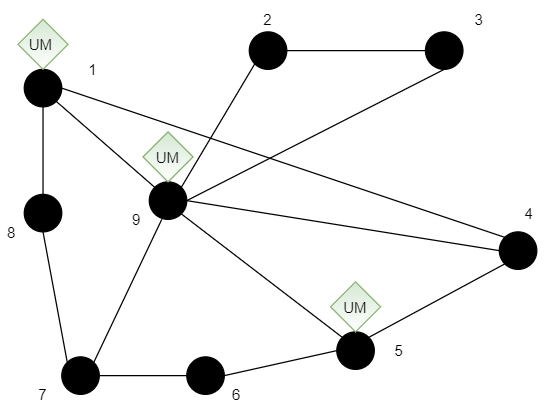
\includegraphics[scale=0.8]{figuras/Rede9_gen.jpg}
		\caption{Rede 9 barras genérica.}
		\label{fig3} % mudar a referencia de acordo com o desejado
	\end{figure}

	A Figura \ref{fig3} apresenta uma forma de representação de uma rede elétrica genérica. As esferas pretas são os barramentos referentes a uma subestação de energia, nessas são inseridas as UMs desejadas. No presente caso, as barras 1, 5 e 9 apresentam UMs alocadas, as quais, sem perda de generalidade, podem ser consideradas completas. Esses barramentos (ou subestações) são conectados por linhas de transmissão, e é exatamente a relação entre a topologia e o plano de medição que determina se uma rede planejada é observável, ou não. Uma breve inspeção dessa rede permite concluir que a mesma é observável, considerando as UMs instaladas completas. Ainda que a rede seja observável, essa pode apresentar criticalidades de medidas diversas. No presente estudo interessa-se em mitigá-las de acordo com um critério de prioridades e com um lote de UMs limitado.
	
	A Figura \ref{fig4} ilustra toda a problemática discorrida até o momento. Nela observa-se um lote genérico de 2 UMs o qual deseja alocar em um conjunto de barras livres BL= (2,3,4,9,7,8). O problema consiste em escolher quais duas barras que melhor solucionam o problema das criticalidades. 
	
	\begin{figure}[H]
		\centering 
		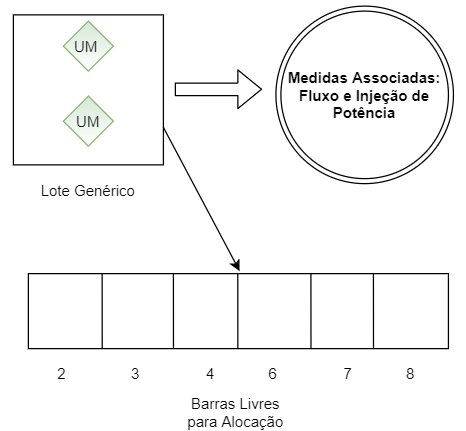
\includegraphics[scale=0.8]{figuras/UMs_aloc.jpg}
		\caption{Ilustração da Problemática.}
		\label{fig4} % mudar a referencia de acordo com o desejado
	\end{figure}
	
	Essa situação é evidentemente combinatorial e apresenta um potencial de crescimento de possibilidades com o aumento do número de barras disponíveis e da relação com o tamanho dos lotes. Isso estará inerente associado à dimensão da rede analisada e do plano de medição inicial considerado. Para ilustrar essa situação basta considerar a rede em questão, para 6 barras disponíveis e um lote de 2 UMs o total de configurações possíveis seriam 15. Considerando um caso maior com 20 barras disponíveis e um lote com 7 UMs, por exemplo, nessa circunstância o problema passaria para a possuir 77520 configurações possíveis. Isso evidencia o crescimento expressivo e combinatorial de acordo com a dimensão do problema e do lote e assim justifica a investigação de uma abordagem através de alguma meta-heurística.
	

\subsection{Formulação Matemática}	

Nas seções anteriores o problema das criticalidades de medidas foi inserido no contexto da Estimação de Estado e a importância da mitigação dessas foi destacada. Também foram explorados os aspectos do problema proposto neste trabalho, o qual envolve a alocação de lotes de UMs afim de minimizar as criticalidades da rede. As premissas e os elementos relacionados ao problema foram explicitados e discutidos. Na presente seção o objetivo é apresentar a formulação matemática proposta para esse problema.

Seja uma rede observável com $\mathbf{n}$ barras, deseja-se mitigar as criticalidades de ordem 1, 2 e 3 dessa rede através da inserção de um lote $\mathbf{L}$ pré-estabelecido de UMs. Para avaliar a qualidade de cada novo plano de medição utiliza-se a seguinte equação:
	
	\begin{equation}
		f_{obj} =  \sum_{k=1}^{kmax}w_k*n_k	\\	
		%f_{obj}= PLOC= Pr(x \in S)= E(f_s(x))
		\label{eq5}
	\end{equation}
	
Na Equação \ref{eq5}  $w_k$ é um vetor de pesos que indica a importância de cada criticalidade por cardinalidade $k$. Ou seja, o peso para as cardinalidades inferiores deve ser maior que para as superiores. Assim sendo, deseja-se priorizar a diminuição de criticalidades de ordens inferiores, mas com uma ponderação que resulte em um equilíbrio na redução dessas. No presente trabalho $n_k$ será o número de criticalidades, por cardinalidade, presentes no sistema após a adição do lote de UMs disponíveis. 

Os valores do vetor $n_k$ são obtidos através de um processo de busca por criticalidades por meio de um algoritmo combinatorial que foge do escopo do presente trabalho, para maiores detalhes é valida a consulta de \cite{AbelTese16} e \cite{BB16}. A Figura \ref{fig5} ilustra simplificadamente essa etapa.Sabendo-se o tamanho do lote e com a garantia de que a rede é observável, o objetivo é minimizar o valor da Equação \ref{eq5}. É importante salientar que os valores de $w_k$ devem ser estabelecidos previamente ao processo de otimização e podem variar de acordo com o tamanho, configuração da rede e plano de medição. No presente trabalho essa determinação foi realizada experimentalmente através de uma inspeção das criticalidades iniciais da rede. Uma metodologia mais completa, que envolva conceitos estatísticos, para a determinação do vetor $w_k$ foi deixada para trabalhos futuros.

\begin{figure}[H]
	\centering 
	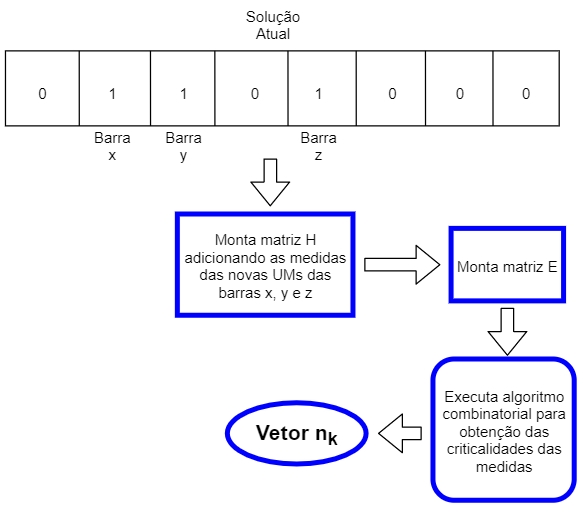
\includegraphics[scale=0.75]{figuras/Gera_nk.jpg}
	\caption{Esquema para obtenção do vetor de criticalidades.}
	\label{fig5} % mudar a referencia de acordo com o desejado
\end{figure}

Por questões de simplificação serão analisadas criticalidades com  $k_{max}$ até o valor 3, sendo no caso da rede 118 barras apenas as cardinalidades 1 e 2. Conforme abordado, a determinação de criticalidades de ordens elevadas é um problema combinatorial difícil e como o mesmo deve ser executado inúmeras vezes ao longo do processo de otimização, o foco serão as criticalidades de ordens inferiores. Isso é justificável pois na prática essas criticalidades (k igual a 1, 2 e 3) são aquelas que tornam a rede mais vulnerável quanto à capacidade de execução de um processo de Estimação de Estado com qualidade, considerando confiabilidade e robustez quanto à presença de erros grosseiros nas medidas. Novamente, os valores dos pesos $w$ foram estabelecidos, de certa forma, empiricamente e precisam ser ajustados para se obter, em uma dada rede, uma relação entre as criticalidades que reflita a prioridade de uma em relação às demais, mas de uma forma equilibrada.

\subsection{Ilustração da Modelagem}

Com a formulação matemática definida pode-se prosseguir para a forma de representação das soluções candidatas ao longo do processo otimização.  Para tal considera-se as etapas genéricas da otimização, definição das entradas, processo e saída.

 \begin{itemize}
 	\item \textbf{Entradas:}
 	\begin{itemize}
 	\item Rede Observável;
 	\item Plano de medição original;
 	\item Quantidade (lote) de unidades de medição (UMs) disponíveis para serem alocadas (por simplificação,todas com mesmo custo e iguais);
 	\item Quantidade de barras na rede disponíveis para a alocação das UMs.
 	\end{itemize}
 \end{itemize}

 \begin{itemize}
	\item \textbf{Processo:}
	\begin{itemize}
		\item Alocação ótima (considerando os critérios e premissas definidos) das UMs disponíveis nas barras que se encontram livres para a inserção;
	\end{itemize}
\end{itemize}


\begin{itemize}
	\item \textbf{Saída:}
	\begin{itemize}
		\item Novo plano de medição com as quantidades de criticalidades prioritárias reduzidas;
	\end{itemize}
\end{itemize}

As Figuras \ref{fig6} e \ref{fig7} ilustram a representação da solução através de um vetor binário com $n$ posições, onde $n$ é a quantidade de barras (barramentos) livres na rede. A solução final será a alocação adequada de um lote limitado de UMs em um subconjunto dessas barras disponíveis. O valor 1 indica a inserção de uma UM, já o valor 0 diz respeito ao contrário.

\begin{figure}[H]
	\centering 
	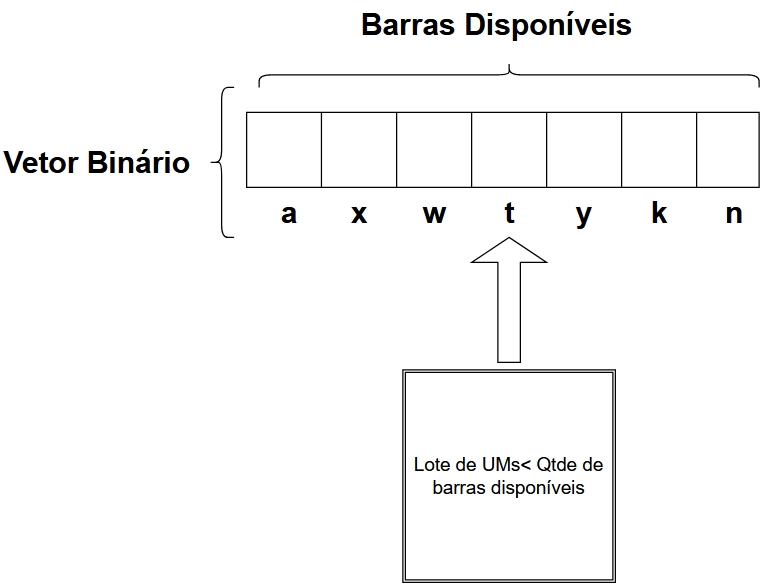
\includegraphics[scale=0.6]{figuras/vetor_bin.jpg}
	\caption{Vetor binário representando as barras disponíveis.}
	\label{fig6} % mudar a referencia de acordo com o desejado
\end{figure}

\begin{figure}[H]
	\centering 
	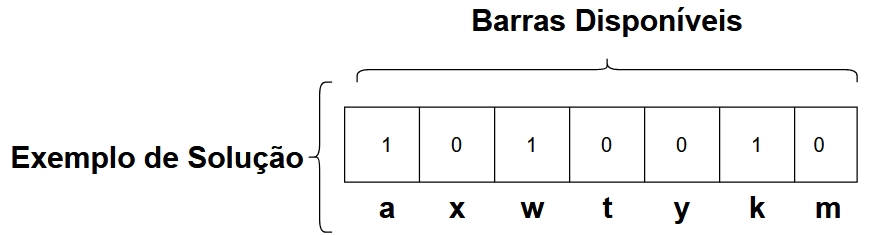
\includegraphics[scale=0.6]{figuras/exemplo_generico.jpg}
	\caption{Exemplo de solução genérica.}
	\label{fig7} % mudar a referencia de acordo com o desejado
\end{figure}

Para cada novo vetor solução $\mathbf{x}$ a determinação do valor da função objetivo deve ser avaliado. Cada posição em que foram alocadas UMs apresenta uma contribuição de novas medidas, formando assim uma nova matriz Jacobiana $\mathbf{H}$. Através dessa obtém-se uma nova matriz de Covariância dos Resíduos $\mathbf{E}$,que deve ser fatorada para a obtenção do número criticalidades de medidas por cardinalidade. De posse desse valor, o cálculo da $f_{obj}$ para a solução candidata é imediata. Nota-se que o processo de determinação de criticalidades insere um maior peso computacional para a avaliação de uma solução. Entretanto, como o problema nesse enfoque é novo e não existe na literatura uma métrica ou indicador que torne esse processo mais simples utilizou-se a formulação discutia para os testes propostos.


\section{GRASP-VND}

Um das meta-heurísticas propostas para a solução do problema em questão envolve a combinação de duas técnicas muito conhecidas da literatura. O  algoritmo GRASP  \cite{GRASP95} que envolve uma etapa construtiva e uma etapa de busca local e o algoritmo VND \cite{VND97} que itera através de estruturas de vizinhança de forma a encontrar soluções de melhor qualidade. Para o presente trabalho esses algoritmos foram combinados de forma que o VND foi utilizado como a estrutura de busca local do algoritmo GRASP. O pseudocódigo segue abaixo:
\begin{itemize}
	\item Procedimento GRASP-VND
	\item Início:
	\begin{enumerate}
		\item $s^* \leftarrow \varnothing$; 
		\item $f(s) \leftarrow fobj condição inicial$;
		\item $Global~tempo_{max} \leftarrow$ Tempo Máximo definido;
		\item $Iter_{max} \leftarrow$ Número Máximo de Iterações;
		\item limite $\leftarrow 0$ 
		\item Enquanto $limite <= Iter_{max}$ e $tempoSim() <= tempo_{max}$ faça
		\item \quad $s' \leftarrow$ ConstruçãoGRASP(f(.),$\alpha$,lote,barrasLivres);
		\item \quad $s'' \leftarrow$ VND($s'$); 
		\item \quad se $f(s'') < f(s^*)$
		\item \qquad  $s^* \leftarrow s''$;
		\item \quad fim-se;
		\item \quad limite= limite +1;
		\item fim-enquanto;
		\item retorna $s^*$;
	\end{enumerate}	
	\item fim GRASP-VND
\end{itemize}

Basicamente a meta-heurística se baseia em duas etapas, a fase construtiva que gera a cada iteração uma solução baseada em alguma métrica ou heurística e a fase de busca local a qual tenta buscar, através de um conjunto de estruturas de vizinhanças, soluções melhores. De acordo com o algoritmo apresentado considerou-se um limite de tempo global para o processo, visto que a avaliação da função objetivo pode ser custosa. Esse tempo global é avaliado ao longo do processo de forma que o procedimento é finalizado imediatamente se esse for atingido. Na sequência a fase de construção será apresentada.

\subsection{Construção GRASP}

 A meta-heurística GRASP apresenta como cerne do seu processo uma fase construtiva a cada nova iteração, conforme apresentado na seção anterior. Essa fase construtiva depende basicamente da função ou heurística que se utiliza para a construção da solução e do valor de um coeficiente $\alpha$. Esse é fundamental para a seleção dos candidatos a elementos formadores da solução, para tal se estabelecem duas listas, uma chamada de LC(Lista de Candidatos) e outra de LRC(Lista Restrita de Candidatos). O algoritmo abaixo generaliza o procedimento de construção:
 
 \begin{itemize}
 	\item Considere $\alpha \in [0,1]$
 	\item ConstruçãoGRASP(f(.),$\alpha$,x,lote,barrasLivres)
 	\item Início:
 	\begin{enumerate}
 		\item $x \leftarrow zeros(barrasLivres)$; 
 		\item Inicializa LC com todos os candidatos ordenada pela função heurística f(.);
 		\item complete=0;
 		\item Enquanto complete $\neq$ 1;
 		\item \quad s-= min$\left \{f(t)/t \in LC \right \}$; 
 		\item \quad s+= máx$\left \{f(t)/t \in LC \right \}$; 
 		\item \quad LRC= $\left \{s \in LC/f(s) \leq s- +\alpha(s+ - s-) \right \}$;
 		\item \quad seleciona um elemento de LRC aleatoriamente;
 		\item \quad Insere o valor 1 em x na posição associada ao barramento selecionado da lista;
 		\item \quad Atualiza LC removendo o barramento selecionado;
 		\item \quad se numElem(x) = lote então
 		\item \qquad complete=1;
 		\item \quad fim-se
 		\item fim-enquanto
 	\end{enumerate}	
 	\item fim Construção
 \end{itemize}

O procedimento de construção acima generaliza o que foi desenvolvido para o presente trabalho. Basicamente uma solução válida para teste é um vetor binário com o número de elementos 1's igual ao tamanho do lote pré-estabelecido. Inicia-se na linha 1 o vetor solução x com todas as posições iguais a 0 e com um tamanho equivalente ao número de UMs disponíveis. Cada posição do vetor está associada a um barramento específico. Assim sendo o procedimento de construção segue enquanto a solução corrente x ainda está incompleta. Forma-se uma LC considerando como f uma função heurística que é basicamente o número de medidas que cada barramento pode disponibilizar para a rede. Ou seja, uma barra com apenas uma única conexão irá possuir f igual a 2, pois pode fornecer duas medidas, uma de fluxo e outra de injeção de potência. Esse valor de f é calculado para cada barra candidata, após isso essas barras são ordenadas para formar a LC. A ordenação para esse trabalho depende da rede e do caso corrente, isso porque de acordo com a configuração da rede, as barras com apenas uma única conexão podem ser consideradas melhores que outras com mais conexões, sendo nesses casos a ordenação crescente. Caso contrário, quando não se possuir informações da rede ou caso não haja barras terminais, ordena-se de forma decrescente. As linhas 5 a 7 do algoritmo basicamente dizem respeito à seleção dos elementos para a LRC. O valor de alfa irá determinar o tamanho da lista restrita, sendo que um alfa próximo de 1 torna o processo mais aleatório, já um alfa próximo de 0 faz com que a construção seja mais gulosa. Após a formação da LRC um de seus elementos é sorteado e inserido na solução parcial x. A LC é atualizada e para o presente trabalho avalia-se o número de elementos iguais a 1 na solução x (função numElem(x)). Caso esse número seja igual ao tamanho lote pré-estabelecido já se tem uma solução completa válida e pode-se finalizar a etapa de construção. Caso contrário parte-se para uma nova iteração e seleção de um próximo elemento. A Figura \ref{fig8} ilustra o conceito de LC e LRC discutido nesse parágrafo. Observa-se que no caso de um alfa muito pequeno praticamente a escolha do elemento será mais gulosa. Na sequência são estabelecidos mais detalhes sobre a etapa de construção.

\begin{figure}[H]
	\centering 
	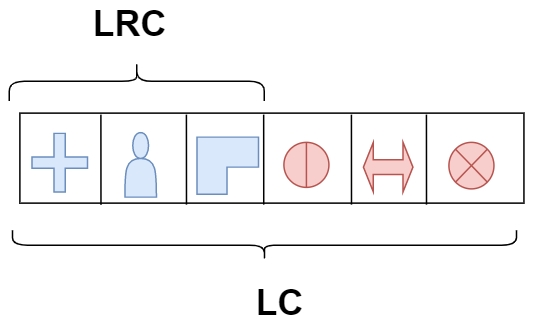
\includegraphics[scale=0.6]{figuras/LC_LRC.jpg}
	\caption{Representação genérica das Listas LC e LRC.}
	\label{fig8} % mudar a referencia de acordo com o desejado
\end{figure}

\subsection{Critérios de Construção}

De acordo com o exposto sobre o processo de determinação das tuplas críticas pode-se concluir que a avaliação da qualidade de uma solução é um processo um pouco custoso e conforme a formulação proposta esse conhecimento é fundamental para a avaliação da função objetivo. Para evitar cálculos excessivos dessas criticalidades a fase de construção do GRASP faz uso de uma heurística estabelecida empiricamente.

Em sistemas elétricos existem barramentos que estão possuem mais conexões com outros, dessa forma a inserção de UMs nesses pode impactar de forma mais ampla as criticalidades presentes nessa rede. Em contrapartida existem casos em que se conhece a rede elétrica e o plano de medição inicial e sabe-se que o mesmo possui inúmeras barras terminais e várias medidas críticas. Nessas situações é mais provável que essas estejam relacionadas a barras conectadas a outras que são terminais. Dessa forma, a inserção de UMs em barras com menos conexões(terminais) pode ser preferível.

Com essas ideias estabeleceu-se os seguintes critérios heurísticos para a etapa de construção e para a consequente formação e ordenação da Lista de Candidatos Restritos:

\begin{enumerate}
	\item Em redes sem barras terminais importantes ou com pouco conhecimento do arranjo das medidas ordena-se a LC dando preferência à inserção de UMs em barras com mais conexões, ou seja, essas estarão no topo da lista;
	
	\item Em redes com barras terminais sem UMs e com muitas criticalidades "próximas" a esses barramentos, então prioriza-se na ordenação da LC as barras com menos conexões;
	
\end{enumerate} 


A Figura \ref{fig9} ilustra essa formação da LC de maneira genérica:

\begin{figure}[H]
	\centering 
	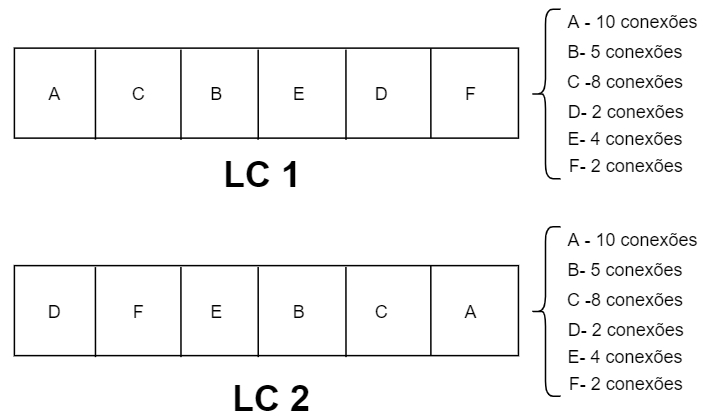
\includegraphics[scale=0.6]{figuras/LC_construct.jpg}
	\caption{Representação da formação da lista restrita de acordo com os critérios.}
	\label{fig9} % mudar a referencia de acordo com o desejado
\end{figure}

De acordo com a Figura \ref{fig9} pode-se entender o procedimento para a construção da lista de candidatos de acordo com os critérios. Caso se considere a condição 1 as barras com mais conexões a lista é ordenada de forma decrescente, caso contrário essa ordenação é realizada de maneira crescente.

\section{VNS-VND}

Na seção anterior foram apresentados os conceitos e as ideias básicas do algoritmo GRASP-VND aplicado na presente proposta. Nessa seção outra metaheurística testada será descrita e definida em respeito ao trabalho em questão. A metaheurística se baseia em um conceito de busca em vizinhança variável, a qual foi apresentada em \cite{VND97}. Basicamente essa técnica perturba de maneira sistemática a solução corrente através de uma ou várias estruturas de vizinhança. Esse processo pode ser útil para promover uma diversificação da busca e fugir de uma possível estagnação. A cada vez que abusca local não é capaz de melhorar a solução corrente altera-se a "perturbação" através da alteração da vizinhança. Essa etapa por vezes pode "piorar" a solução atual, mas através dela é possível escapar de alguns ótimos locais. O VNS-VND proposto realiza, primeiramente, uma etapa de geração de uma solução inicial viável. Com essa inicia-se o processo iterativo referente ao VNS, enquanto não se atingir um limite de iterações ou de tempo máximo, realiza-se uma perturbação na melhor solução atual e parte-se para a etapa de busca-local (VND) análoga aquela proposta no GRASP-VND. Após a busca-local compara-se a melhor solução obtida com a aquela de melhor fitness até o momento. Caso a nova solução seja superior atualiza-se a \textit{best solution} e retorna-se à vizinhança inicial do VNS, caso contrário incrementa-se a vizinhança. Uma iteração é finalizada ao serem testadas todas as vizinhanças pré-estabelecidas. O algoritmo na sequência implementa os passos que foram descritos.

\begin{itemize}
	\item Procedimento VNS-VND 
	\item Início:
	\begin{enumerate}
		\item $s \leftarrow GerSolInicial()$; 
		\item $max_{iter} \leftarrow 0$;
		\item $lim_{iter} \leftarrow$ input("Insere Limite Iterações");
		\item $Global~tempo_{max} \leftarrow$ input("Insere Limite Tempo");
		\item Enquanto $max_{iter} \leq lim_{iter}$ e $tempoSim() < tempo_{max}$   faça
		\item $k \leftarrow 1$;
		\item Enquanto $k \leq k_{max}$ e $tempoSim() < tempo_{max}$ faça
		\item \quad $s'\leftarrow$ Vizinho Aleatório de $N_k(s)$;
		\item \quad $s'' \leftarrow VND(s')$; 
		\item \quad se $f(s'') < f(s)$
		\item \qquad  $s \leftarrow s''$;
		\item \qquad  $k \leftarrow 1$;
		\item \quad senão $k \leftarrow k + 1$;
		\item \quad fim-se;
		\item fim-enquanto;
		\item fim-enquanto;
		\item retorna $s$;
	\end{enumerate}	
	\item fim VNS-VND
\end{itemize}

O procedimento que caracteriza essa metaheurística é a etapa estabelecida na linha 8. Essa função gera um vizinho aleatório da solução corrente de acordo com a estrutura de vizinhança k atual. Diferentemente da busca local (VND) essa etapa gera um vizinho qualquer, seja ele melhor ou pior que a solução corrente. A inserção dessa etapa tem o objetivo percorrer diversas regiões do espaço de busca, possibilitando uma diversificação das soluções testadas. O vizinho gerado é então enviado para a etapa de busca local (VND) na qual busca-se encontrar uma solução com qualidade superior.



\subsection{Soluções Iniciais}
Conforme apresentado na seção anterior o algoritmo VNS-VND depende de uma solução inicial que será "modificada" ao longo das iterações realizadas. A forma de geração dessa solução pode acelerar a convergência para boas soluções. Para o presente trabalho foram testadas duas estratégias para obtenção de soluções iniciais:

\begin{itemize}
	\item \textbf{Solução Inicial Aleatória} - Constrói-se de forma sistemática uma alocação viável de UMs através do sorteio aleatório das barras nas quais será distribuído o lote disponível, esse tipo de solução pode ser interessante quando se conhece pouco da rede ou necessita-se de diversificação.
	
	\item \textbf{Solução Inicial Gulosa} - Gera-se uma solução inicial com um critério guloso baseado na quantidade de conexões presentes em cada barramento, as escolhas desse critério seguem as mesmas premissas da formação da lista de candidatos do algoritmo GRASP-VND. Esse forma de geração possibilita a inserção de informações quanto às barras disponíveis para alocação.
\end{itemize}
	


\section{Estruturas de Vizinhança e Busca Local}

De acordo com o exposto ambas metaheurísticas aplicadas ao problema de minimização das criticalidades utilizam-se de uma etapa de busca local. Para o presente trabalho foram desenvolvidas quatro estruturas de vizinhança elementares. A ideia geral é que as vizinhanças de cardinalidades menores sejam menos "distantes" que as maiores. Basicamente as estruturas desenvolvidas se baseiam em trocas e rotações do vetor binário representativo da solução. As vizinhanças aplicadas foram as seguintes:

\begin{itemize}
	\item \textbf{Vizinhança 1} - Baseia-se na troca de uma posição igual a 1 na solução por outra igual a 0, ou seja, retira a UM de uma barra e coloca-se em outra disponível.
	\item \textbf{Vizinhança 2} - Realiza-se a troca de duas posições iguais a 1 por outras duas iguais a 0;
	\item \textbf{Vizinhança 3} - Aplica-se a vizinhança 1 e rotaciona-se o vetor binário;
	\item \textbf{Vizinhança 4} - Aplica-se a vizinhança 2 e rotaciona-se o vetor binário;
\end{itemize}

Para a análise das vizinhanças os algoritmos desenvolvidos avaliam diversas soluções e por fim seleciona-se aquela de melhor qualidade. Conforme será discutido, em redes menores é viável a a avaliação de todos os vizinhos. Entretanto, em redes um pouco maiores essa busca se torna muito custosa tanto pela quantidade de vizinhos quanto pelo tempo despendido para o cálculo das criticalidades. Nesses casos serão avaliados apenas uma porção dos vizinhos da solução corrente. Para essas situações realiza-se uma busca "pseudo-aleatória", isso porque sorteia-se as posições que serão trocadas, mas conforme esses sorteios são realizados há o cuidado para que soluções iguais não sejam recalculadas e ou geradas. Para isso sorteia-se apenas parte dos elementos a serem trocados, após esse primeiro sorteio as trocas realizam-se deterministicamente até se esgotarem as possibilidades de combinações. A Figura \ref{fig10} apresenta uma ilustração de como realiza-se as buscas parciais nas vizinhanças. No caso de apenas uma troca sorteia-se um elemento ativo e realiza-se as trocas desse pelas posições vazias. Após todas as trocas esse elemento ativo é removido da continuidade do processo, esse processo continua até se realizar um limite máximo de trocas estabelecido. No caso de duas trocas o processo é mais difícil mas realiza-se um primeiro sorteio no qual seleciona-se um elemento ativo. O segundo elemento a ser desligado não é sorteado, itera-se por todos os ativos combinando-os com o primeiro sorteado. Em relação às posições de troca sorteia-se a primeira troca, as demais são determinísticas. No caso itera-se pelas outras posições disponíveis combinando-as duas a duas com a primeira sorteada. Esse processo segue até que sejam realizadas todas as combinações possíveis duas a duas com a o primeiro elemento ativo sorteado. Ao fim desse processo essa posição é bloqueada para evitar repetições. O processo segue enquanto não se atingir o limite de vizinhos pré-determinado.

\begin{figure}[H]
	\centering 
	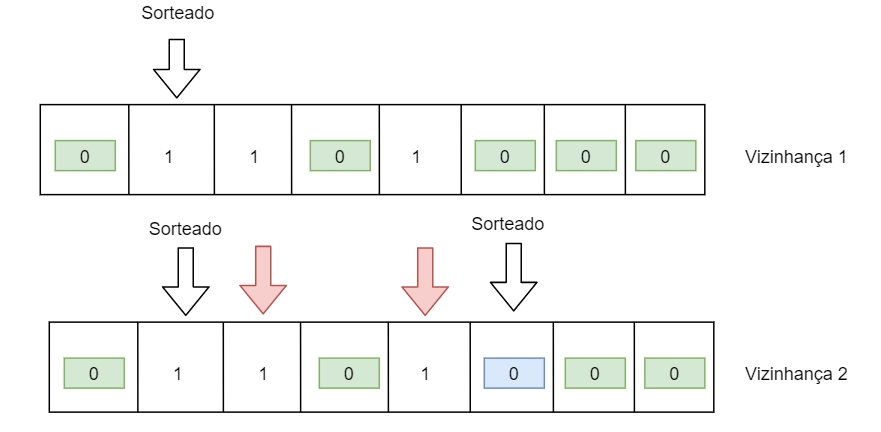
\includegraphics[scale=0.6]{figuras/Vizinhancas.jpg}
	\caption{Representação simplificada do processo de busca parcial nas vizinhanças.}
	\label{fig10} % mudar a referencia de acordo com o desejado
\end{figure}


\subsection{VND}

A heurística chamada de VND(Variable Neighborhood Descent) é um método utilizado amplamente nas etapas de buscas locais. O procedimento se baseia, basicamente, em uma troca sistemática de estruturas vizinhanças de maneira a se encontrar uma solução de melhor qualidade. O algoritmo permanece em uma estrutura de vizinhança buscando melhorar uma solução corrente, quando não se consegue isso parte-se para outra vizinhança. Sempre que uma melhor solução é encontrada, dentro de um limite de vizinhanças, retorna-se para a vizinhança inicial. O algoritmo é finalizado quando todas as vizinhanças foram exploradas e não se conseguiu melhora da solução corrente ou quando se atinge um limite de tempo máximo da execução global das metaheurísticas GRASP-VND ou VNS-VND.

No presente trabalho foram utilizadas 4 estruturas de vizinhança. Para redes menores e menos custosas é possível avaliar a vizinhança completa de uma solução corrente, garantindo assim que o melhor vizinho é um ótimo local para aquela vizinhança em relação à solução corrente. Em contrapartida, como o cálculo da função objetivo se torna mais custoso com o crescimento da rede e, além disso, o número de combinações por vizinhança também cresce, para a redes mais pesadas avalia-se parcialmente um subconjunto desses vizinhos. Nesse caso o procedimento não garante que se obteve um ótimo local mas possibilita ao algoritmo reduzir o tempo consumido em apenas uma única vizinhança.

O algoritmo na sequência generaliza a etapa de VND, que é a etapa de busca local das metaheurísticas testadas. No caso de uma busca parcial o que se realiza é uma limitação do número de iterações por vizinhança e seleciona-se uma parcela dos possíveis vizinhos ao longo dessas iterações. 

\begin{itemize}
	\item Procedimento VND(s) 
	\item Início:
	\begin{enumerate}
		\item $k_{max} \leftarrow 4$; 
		\item $k \leftarrow 1$;
		\item Enquanto $k \leq k_{max}$ e $tempoSim()$<$tempo_{max}$ faça
		\item \quad Encontrar melhor vizinho s' (ou o melhor dentro de um limite) $\in N_k(s)$; 
		\item \quad se $f(s') < f(s)$
		\item \qquad  $s \leftarrow s'$;
		\item \qquad  $k \leftarrow 1$;
		\item \quad senão $k \leftarrow k + 1$;
		\item \quad fim-se;
		\item fim-enquanto;
		\item retorna $s$;
	\end{enumerate}	
	\item fim VND
\end{itemize}



\section{Hash Global Auxiliar}
As metaheurísticas desenvolvidas para explorar o presente problema apresentam uma etapa sistemática de busca local. Essa envolve, a cada geração de um vizinho, o cálculo do valor da função objetivo, para tal necessita-se executar um algoritmo de determinação de criticalidades de medidas. Esse apresenta uma natureza combinatorial e realiza diversas fatorações matriciais para a obtenção das criticalidades. É evidente que esse processo, ainda que desenvolvido de maneira eficiente, pode ser dispendioso e se evitado seria de grande valia para a eficiência do algoritmo. Sabendo-se que os algoritmos GRASP e VNS são apresentam originalmente mecanismos de memória de longo prazo,através das iterações realizadas, propõem-se então inserir esse mecanismo no processo. O objetivo dessa inserção é evitar-se a repetição de cálculos de criticalidades em possíveis candidatos já explorados em alguma iteração anterior. Essa proposta é preliminar e pode ser aprimorada com outras estratégias de memória adicionais como listas Tabu. Entretanto, para o trabalho utilizou-se a estrutura de dados conhecida como tabela Hash.

Uma tabela Hash é uma estrutura de dados extremamente utilizada em situações em que se deseja consultar se alguma informação ou cliente já se encontra cadastrado e caso esteja possibilita a consulta dos dados no melhor caso em tempo constante. Para essa implementação utilizou-se a estrutura "Map" presente na plataforma MATLAB\textregistered. A tabela desenvolvida apresenta dois atributos básicos, o primeiro uma chave chave e o segundo  um conteúdo armazenado. A Figura \ref{fig11} apresenta uma ilustração referente a essa tabela.

\begin{figure}[H]
	\centering 
	\includegraphics[scale=0.7]{figuras/Hash_table.jpg}
	\caption{Tabela Hash desenvolvida.}
	\label{fig11} % mudar a referencia de acordo com o desejado
\end{figure}

A tabela Hash inicia-se vazia e ao decorrer das iterações, para ambas metaheurísticas, essa é preenchidas. A chave para acessar uma posição da tabela é uma string binária referente ao vetor solução produzido. O conteúdo armazenado é um vetor que concatena duas informações importantes, e que são o ponto chave da aplicação da Hash, o valor da função objetivo e um vetor com as criticalidades dos sistema corrente. Quando uma solução é inédita essa é inserida na Hash, caso contrário o algoritmo se utiliza da informação previamente avaliada e evita-se o recalculo da função objetivo. Para mais detalhes quanto aos conceitos e tipos de tabela Hash recomenda-se a leitura de \cite{Cormen}.

\section{Testes}

Para os testes utilizou-se uma máquina com configuração Intel i7 sétima geração e 16 Gb de memória RAM. O algoritmo para computação das tuplas críticas foi desenvolvido na linguagem C utilizando-se OpenMP para paralelizar o processo nos núcleos da CPU. As etapas de processamento da topologia da rede, construção das matrizes elementares, além das metaheurísticas GRASP-VND e VNS-VND foram implementadas através do software MATLAB\textregistered. O foco nos testes não foi desempenho mas sim analisar a qualidade da solução obtida nas simulações, de forma a comparar se foram equivalentes ou se alguma das metaheurísticas testadas se sobressai frente aos casos analisados. Além disso o objetivo é se obter uma maior sensibilidade sobre o problema proposto para maiores aprimoramentos das estratégias propostas.

Os sistemas escolhidos para testes foram as redes IEEE 30 e 118 barras extraídas respectivamente de \cite{BB16} e \cite{Quant13}, os quais se referem ao processo de análise das criticalidades de sistema de medição. O plano de medição utilizado para a topologia com 30 barras foi ligeiramente modificado em relação ao proposto em \cite{BB16}, isso porque desejava-se uma maior quantidade de medidas críticas iniciais. Para tal foram removidas as medidas A3, P9, P3, P10, P12, P27, onde A3 é uma medida de ângulo e as demais são injeções de potência ativa na rede. As medidas removidas estão marcadas na Figura \ref{fig12}. Em relação à rede de 118 barras utilizou-se o mesmo plano de medição apresentado em \cite{Quant13}, com o objetivo de se avaliar a condição onde existem medidas críticas associadas a barras terminais, esse plano, apresentado na Figura \ref{fig13}, será referenciado como plano 118 base.


\begin{figure}[H]
	\centering 
	\includegraphics[scale=0.7]{figuras/Rede30bus.jpg}
	\caption{Rede IEEE 30 Barras.\cite{BB16}}
	\label{fig12} % mudar a referencia de acordo com o desejado
\end{figure}

\begin{figure}[H]
	\centering 
	\includegraphics[scale=0.8]{figuras/Rede118bus.jpg}
	\caption{Rede IEEE 118 Barras.\cite{Quant13}}
	\label{fig13} % mudar a referencia de acordo com o desejado
\end{figure}

Para se avaliar uma condição mais complexa para alocação de UMs desenvolveu-se um plano de medição alternativo, observável, para a rede 118 barras. Esse é composto por 39 UMs completas resultando em 79 barramentos livres para alocações de um futuro lote de UMs. Para a geração desse plano inicial utilizou-se a modelagem proposta por \cite{Gou08_1}, a qual utiliza os conceitos de programação linear para a obtenção de um plano de medição observável. A solução do problema foi obtida através de uma função de programação linear inteira. A nova configuração da rede não será apresentada por questões de espaço.

Os testes que serão apresentados podem ser sintetizados da seguinte maneira:

\begin{itemize}
	\item \textbf{Rede 30 Barras}- Lotes de UMs de tamanho 3 e 6; $k_{max}=3$ e 12 barramentos disponíveis para alocação;

	\item \textbf{Rede 118 Barras plano base}- Lotes de UMs de tamanho 6 e 9; $k_{max}=2$ e 19 barramentos disponíveis para alocação;

	\item \textbf{Rede 118 Barras Nova}- Lote de tamanho 10, $k_{max}=2$ e 79 barramentos disponíveis para alocação;
\end{itemize}

As Tabelas abaixo sintetizam os principais testes realizados. A Tabela \ref{tab4} apresenta um teste alternativo para a rede 118 barras com nova configuração de medidas, esse avalia as melhores configurações obtidas nos testes da Tabela \ref{tab3} com tempo máximo reduzido.


\begin{table}[H]
	\scalefont{0.70}
	\centering
	\caption{Critérios dos testes Rede IEEE 30 barras.}
	\begin{tabular}{|c|c|c|c|c|c|c|}
		\hline
		\textbf{Técnica} & \textbf{Alfa} & \textbf{Sol. Inical} & \textbf{Tempo Máx} & \textbf{Iter. Máx} & \textbf{Busca Local} & \textbf{Nº de Testes} \\
		\hline
		GRASP-VND & 0,3;0,5;0,8 & -     & 10 min & 5    & Completa & 3 \\
		\hline
		VNS-VND & -     & Gulosa e Aleatória & 10 min & 5    & Completa & 3 \\
		\hline
	\end{tabular}%
	\label{tab1}%
\end{table}%


\begin{table}[H]
	\scalefont{0.70}
	\centering
	\caption{Critérios dos testes Rede IEEE 118 barras Base.}
	\begin{tabular}{|c|c|c|c|c|c|c|}
		\hline
		\textbf{Técnica} & \textbf{Alfa} & \textbf{Sol. Inical} & \textbf{Tempo Máx} & \textbf{Iter. Máx} & \textbf{Busca Local} & \textbf{Nº de Testes} \\
		\hline
		GRASP-VND & 0,3;0,5;0,8 & -     & 45 min & 15    & Parcial & 3 \\
		\hline
		VNS-VND & -     & Gulosa e Aleatória & 45 min & 15    & Parcial & 3 \\
		\hline
	\end{tabular}%
	\label{tab2}%
\end{table}%

% Table generated by Excel2LaTeX from sheet 'Planilha1'
\begin{table}[H]
	\scalefont{0.70}
	\centering
	\caption{Critérios dos testes Rede IEEE 118 barras Nova.}
	\begin{tabular}{|c|c|c|c|c|c|c|}
		\hline
		\textbf{Técnica} & \textbf{Alfa} & \textbf{Sol. Inical} & \textbf{Tempo Máx} & \textbf{Iter. Máx} & \textbf{Busca Local} & \textbf{Nº de Testes} \\
		\hline
		GRASP-VND & 0,3;0,8   & -     & 2:30h & 50    & Parcial & 3 \\
		\hline
		VNS-VND & -     & Gulosa e Aleatória & 2:30h & 50    & Parcial & 3 \\
		\hline
	\end{tabular}%
	\label{tab3}%
\end{table}%

\begin{table}[H]
	\scalefont{0.70}
	\centering
	\caption{Critérios dos testes Rede IEEE 118 barras Nova.}
	\begin{tabular}{|c|c|c|c|c|c|c|}
		\hline
		\textbf{Técnica} & \textbf{Alfa} & \textbf{Sol. Inical} & \textbf{Tempo Máx} & \textbf{Iter. Máx} & \textbf{Busca Local} & \textbf{Nº de Testes} \\
		\hline
		GRASP-VND & Melhor Config.   & -     & 30 min & 15    & Parcial & 5 \\
		\hline
		VNS-VND & -     & Melhor Config. & 30 min & 15    & Parcial & 5 \\
		\hline
	\end{tabular}%
	\label{tab4}%
\end{table}%

Foram estabelecidos tempos limites para cada teste das técnicas implementadas, além disso nas redes 118 barras foi limitado o número total de vizinhos analisados em cada vizinhança. Para os testes apresentados nesse artigo esse limite definido empiricamente foi de 50 vizinhos. No caso da rede IEEE 118 barras, com plano modificado, como os testes são mais dispendiosos e a quantidade de possibilidades de configurações é elevada utilizou-se nos testes condições extremas para o GRASP-VND e para o VNS-VND. Além disso, considerou-se um limite de tempo máximo maior para os 3 testes, visto que a dimensão de soluções se encontra na ordem de $1 \times 10^{12}$ configurações possíveis. A escolha da cardinalidade máxima igual a 2 para as redes IEEE 118 se deu pelo maior dispêndio de tempo, nos testes preliminares, para o cálculo das criticalidades nessa dimensão de rede. Para as redes IEEE 30 e 118 base foi executado um algoritmo de busca exaustiva para se comparar os resultados das metaheurísticas e se justificar a validade dessas. Para o caso da rede IEEE 118 base limitou-se o tempo da busca exaustiva para 90 minutos e comparou-se o melhor resultado dessa com o das metaheurísticas testadas.

As redes utilizadas apresentam algumas condições iniciais que devem ser melhoradas com o processo de otimização. Essas estão relacionadas à quantidade de tuplas críticas de medidas por cardinalidade desejada. A Tabela \ref{tab5} apresenta a distribuição dessas tuplas críticas por cardinalidade:

\begin{table}[H]
	\scalefont{0.75}
	\centering
	\caption{Distribuição das Criticalidades Iniciais}
	\begin{tabular}{|c|c|c|c|}
		\hline
		\textbf{Rede } & \textbf{Ck1} & \textbf{Ck2} & \textbf{Ck3} \\
		\hline
		30 Barras &       &       &  \\
		\hline
		118 Barras Base &       &       & - \\
		\hline
		118 Barras Modificado &   0     & 97       &  - \\
		\hline
	\end{tabular}%
	\label{tab5}%
\end{table}%

Com o conhecimento dessas criticalidades iniciais, e sabendo-se das prioridades de uma criticalidade de ordem inferior em relação às superiores, estabeleceu-se empiricamente os pesos $w_k$ utilizados para a avaliação da função objetivo, esses são os seguintes:
\begin{itemize}
	\item Rede 30 Barras - $w=[10~3~1.5]$ 
	\item Rede 118 Barras Base - $w=[20~1.5]$ 
	\item Rede 118 Barras Modificado - $w=[1~1]$ 
\end{itemize}

\section{Resultados}

Na sequência os resultados obtidos estão apresentados para a rede IEEE 30 e para as redes IEEE 118. Para as instâncias menores as melhores soluções foram comparadas com os resultados de um algoritmo de busca exaustiva simples. Como não há instâncias de teste na literatura os resultado são preliminares e a comparação foi realizada entre as metaheurísticas e a busca exaustiva em alguns casos.

A Tabelas \ref{tab6} a \ref{tab9} se referem ao teste para a rede 30 barras e lote de tamanho 3. Observa-se que tanto do GRASP-VND quando no VNS-VND as melhores soluções foram as mesmas. Nos testes realizados houve a convergência para esse valor ótimo na primeira iteração para todos eles e por isso o caminho das soluções não foi plotado. Nota-se que esse valor é de fato ótimo pois a Tabela \ref{tab8} indica o resultado de uma busca exaustiva por todas as combinações possíveis de UMs alocadas. Nessa o melhor resultado foi o valor 129 que é exatamente o valor encontrado pelas metaheurísticas. Além disso o tempo para executar essa busca completa equivale-se aos tempos médios dos testes o que já apresenta outro ponto positivo do uso das metaheurísticas. A Tabela \ref{tab9} indica as barras para alocação do lote e as respectivas criticalidades finais do novo plano de medição.

% Table generated by Excel2LaTeX from sheet '30_Lote3_6'
\begin{table}[H]
	\scalefont{0.7}
	\centering
	\caption{Resultados GRASP-VND rede 30 barras (lote=3).}
	\begin{tabular}{|c|c|c|c|}
		\hline
		\textbf{Alfa} & \textbf{Tempo Tot. Médio(s)} & \textbf{Qtd. Iterações} & \textbf{Melhor Sol.} \\
		\hline
		0,3   & 81,2  & 5     & 129 \\
		\hline
		0,5   & 79,1  & 5     & 129 \\
		\hline
		0,8   & 80,7  & 5     & 129 \\
		\hline
	\end{tabular}%
	\label{tab6}%
\end{table}%

% Table generated by Excel2LaTeX from sheet '30_Lote3_6'
\begin{table}[H]
	\scalefont{0.7}
	\centering
	\caption{Resultados VNS-VND rede 30 barras (lote=3).}
	\begin{tabular}{|c|c|c|c|}
		\hline
		\textbf{Sol. Inicial} & \textbf{Tempo Tot. Médio(s)} & \textbf{Qtd. Iterações} & \textbf{Melhor Sol} \\
		\hline
		Aleatória & 88,6  & 5     & 129 \\
		\hline
		Gulosa & 89,4  & 5     & 129 \\
		\hline
	\end{tabular}%
	\label{tab7}%
\end{table}%


% Table generated by Excel2LaTeX from sheet '30_Lote3_6'
\begin{table}[H]
	\scalefont{0.7}
	\centering
	\caption{Resultados busca exaustiva rede 30 barras (lote=3).}
	\begin{tabular}{|c|c|c|}
		\hline
		\textbf{Técnica} & \textbf{Tempo Total(s)} & \textbf{Melhor Sol.} \\
		\hline
		Busca Exaustiva & 80,9  & 129 \\
		\hline
	\end{tabular}%
	\label{tab8}%
\end{table}%

% Table generated by Excel2LaTeX from sheet '30_Lote3_6'
\begin{table}[H]
	\scalefont{0.7}
	\centering
	\caption{Alocação ótima rede 30 barras (lote=3).}
	\begin{tabular}{|l|c|c|}
		\hline
		\multicolumn{1}{|c|}{\textbf{Tupla Binária}} & \textbf{Barras Equivalentes} & \multicolumn{1}{l|}{\textbf{Criticalidades}} \\
		\hline
		0 0 0 0 0 0 1 1 0 1 0 0 & 17|20|26 & 6|6|34 \\
		\hline
	\end{tabular}%
	\label{tab9}%
\end{table}%

As Tabelas \ref{tab10} a \ref{tab13} apresentam os resultados para os testes da rede 30 barras com um lote de tamanho 6 de UMs. Assim como no teste anterior houve a convergência para uma mesma solução ótima nos testes realizados. Em todos os testes as metaheurísticas se mostraram equivalentes e convergiram para um mesmo valor na primeira iteração e por isso os caminhos das soluções não foi plotado. Ao serem confrontadas com um método exaustivo que testa todas as possibilidade alocação das UMs concluis-se que ambas metaheurísticas conseguiram alcançar o melhor valor possível. Além disso, nessa configuração as metaheurísticas foram mais rápidas que o método exaustivo. Isso corrobora para a justificativa de que conforme as instâncias se tornam mais difíceis as metaheurísticas são uma forma inteligente de se buscar soluções de boa qualidade. Por fim, a Tabela \ref{tab13} apresenta a melhor alocação encontrada para as UMs.

% Table generated by Excel2LaTeX from sheet '30_Lote3_6'
\begin{table}[H]
	\scalefont{0.7}
	\centering
	\caption{Resultados GRASP-VND rede 30 barras (lote=6).}
	\begin{tabular}{|c|c|c|c|}
		\hline
		\textbf{Alfa} & \textbf{Tempo Tot.  Médio(s)} & \textbf{Qtd. Iterações} & \textbf{Melhor Sol.} \\
		\hline
		0,3   & 238,2 & 5     & 86,5 \\
		\hline
		0,5   & 232,3 & 5     & 86,5 \\
		\hline
		0,8   & 203,7 & 5     & 86,5 \\
		\hline
	\end{tabular}%
	\label{tab10}%
\end{table}%

% Table generated by Excel2LaTeX from sheet '30_Lote3_6'
\begin{table}[H]
	\scalefont{0.7}
	\centering
	\caption{Resultados VNS-VND rede 30 barras (lote=6).}
	\begin{tabular}{|c|c|c|c|}
		\hline
		\textbf{Sol. Inicial} & \textbf{Tempo Tot. Médio(s)} & \textbf{Qtd. Iterações} & \textbf{Melhor Sol } \\
		\hline
		Aleatória & 249,2 & 5     & 86,5 \\
		\hline
		Gulosa & 262,3 & 5     & 86,5 \\
		\hline
	\end{tabular}%
	\label{tab11}%
\end{table}%

% Table generated by Excel2LaTeX from sheet '30_Lote3_6'
\begin{table}[H]
	\scalefont{0.7}
	\centering
	\caption{Resultados busca exaustiva rede 30 barras (lote=6).}
	\begin{tabular}{|c|c|c|}
		\hline
		\textbf{Técnica} & \textbf{Tempo Total(s)} & \textbf{Melhor Sol.} \\
		\hline
		Busca Exaustiva & 400,4 & 86,5 \\
		\hline
	\end{tabular}%
	\label{tab12}%
\end{table}%


% Table generated by Excel2LaTeX from sheet '30_Lote3_6'
\begin{table}[H]
	\scalefont{0.7}
	\centering
	\caption{Alocação ótima rede 30 barras (lote=6).}
	\begin{tabular}{|l|c|c|}
		\hline
		\multicolumn{1}{|c|}{\textbf{Tupla Binária}} & \textbf{Barras Equivalentes} & \multicolumn{1}{l|}{\textbf{Criticalidades}} \\
		\hline
		0 0 0 0 1 1 1 1 0 1 0 1 & 11|13|17|20|26|30 & 1|12|27 \\
		\hline
	\end{tabular}%
	\label{tab13}%
\end{table}%


Na sequência, as Tabelas \ref{tab14} a \ref{tab17} apresentam os resultados dos testes para a rede 118 barras base e lote de tamanho 6. Nesse teste o crescimento da rede passa a impactar no dispêndio de tempo na execução das metaheurísticas. Apesar disso todos os testes convergiram para um mesmo valor de melhor solução. Nesses testes ambas metaheurísticas foram equivalentes em qualidade de solução, entretanto nota-se que as iterações da técnica VNS-VND foram mais lentas que as do GRASP-VND, isso pode ser observado pela quantidade média de iterações. Ambas metaheurísticas despenderam o tempo máximo pré-estabelecido para as execuções, porém as convergências para o valor ótimo ocorreram nas primeiras iterações dos testes. Os caminhos das solução não foram plotados por questões de espaço, mas em testes futuros é possível estabelecer um tempo máximo inferior devido a essa rápida convergência. Em relação à busca exaustiva pode-se notar que a mesma utilizou todo o tempo máximo pré-estabelecido e ainda assim não alcançou um resultado superior ao das metaheurísticas testadas, mais uma vez corroborando para o uso dessas. Diferentemente dos testes anteriores, nesse foram encontradas 4 configurações distintas, para as UMs, que alcançam um mesmo valor para as criticalidades avaliadas. Isso de fato é possível visto que não se estabeleceu um critério auxiliar para diferenciar essa soluções nessas situações, esse pode ser avaliar a cardinalidade seguinte ou encontrar uma métrica que qualifique cada configuração, mas esses são problemas em aberto e são focos de trabalhos futuros. Apesar de não se saber diferenciar essas configurações, uma rápida mineração dos resultados indica que certas UMs devem estar instaladas em algumas barras específicas na solução final, impactando na redução das criticalidades. Essas seriam, respectivamente, as barras 73, 111 e 116, uma rápida inspeção na topologia da rede indica que essas barras são terminais e impactam diretamente medidas críticas.
% Table generated by Excel2LaTeX from sheet '118_base_lote6e9'
\begin{table}[H]
	\scalefont{0.7}
	\centering
	\caption{Resultados GRASP-VND rede 118 barras base (lote=6).}
	\begin{tabular}{|c|c|c|c|}
		\hline
		\textbf{Alfa} & \textbf{Tempo Tot. Med(s)} & \textbf{Qtd. Média Iterações} & \textbf{Melhor Sol.} \\
		\hline
		0,3   & 2.649 & 14    & 196,5 \\
		\hline
		0,5   & 2.700 & 9     & 196,5 \\
		\hline
		0,8   & 2.700 & 8     & 196,5 \\
		\hline
	\end{tabular}%
	\label{tab14}%
\end{table}%

% Table generated by Excel2LaTeX from sheet '118_base_lote6e9'
\begin{table}[H]
	\scalefont{0.7}
	\centering
	\caption{Resultados VNS-VND rede 118 barras base (lote=6).}
	\begin{tabular}{|c|c|c|c|}
		\hline
		\textbf{Sol. Inicial} & \textbf{Tempo Tot. Med(s)} & \textbf{Qtd. Média Iterações} & \textbf{Melhor Sol.} \\
		\hline
		Aleatória & 2.700 & 2     & 196,5 \\
		\hline
		Gulosa & 2.700 & 2     & 196,5 \\
		\hline
	\end{tabular}%
	\label{tab15}%
\end{table}%

% Table generated by Excel2LaTeX from sheet '118_base_lote6e9'
\begin{table}[H]
	\scalefont{0.7}
	\centering
	\caption{Resultados busca exaustiva rede 118 barras base (lote=6).}
	\begin{tabular}{|c|c|c|c|}
		\hline
		\textbf{Técnica} & \textbf{Tempo Total(s)} & \textbf{Melhor Sol.} & \textbf{Criticalidades} \\
		\hline
		Busca Exaustiva & 5400  & 212   & 4|88 \\
		\hline
	\end{tabular}%
	\label{tab16}%
\end{table}%

% Table generated by Excel2LaTeX from sheet '118_base_lote6e9'
\begin{table}[H]
	\scalefont{0.7}
	\centering
	\caption{Alocações ótimas rede 118 barras base (lote=6).}
	\begin{tabular}{|l|c|c|}
		\hline
		\multicolumn{1}{|c|}{\textbf{Tupla Binária}} & \textbf{Barras Equivalentes} & \multicolumn{1}{l|}{\textbf{Criticalidades}} \\
		\hline
		1000001100001100100 & 10|73|87|111|112|116 & 3|91 \\
		\hline
		0000001100001100110 & 73|87|111|112|116|117 & 3|91 \\
		\hline
		1000001000001100110 & 10|73|111|112|116|117 & 3|91 \\
		\hline
		1000001100001000110 & 10|73|87|111|116|117 & 3|91 \\
		\hline
	\end{tabular}%
	\label{tab17}%
\end{table}%

As Tabelas \ref{tab18} a \ref{tab21} apresentam os resultados dos testes das metaheurísticas para a rede IEEE 118 base e lote de tamanho 9. Novamente ambas metaheurísticas conseguiram alcançar um mesmo valor referente às suas melhores soluções. Por questões de espaço os caminhos das soluções não foram plotados porém houve convergência para o valor 152,5 na primeira iteração dos testes. Isso pode ser explicado pela dificuldade da instância não ser tão elevada e também pela etapa de busca local apresentar várias estruturas de vizinhança. Em relação ao tempo médio das execuções, todos os testes despenderam o tempo máximo 45 minutos (2700 s), entretanto como a convergência ocorreu na primeira iteração dos testes esse tempo pode ser reduzido. É válido salientar que a metaheurística VNS-VND consome um tempo consideravelmente superior ao GRASP-VND em suas iterações. Apesar de terem chegado a um mesmo resultado, o GRASP-VND possui iterações mais rápidas. Esse tempo despendido também está relacionado ao custo envolvido no cálculo da função objetivo e será alvo de melhorias em testes futuros. A Tabela \ref{tab20} apresenta o melhor resultado obtido em uma execução da busca exaustiva, utilizando o dobro do tempo dos testes realizados por ambas metaheurísticas conseguiu-se uma solução de pior qualidade. Mais uma vez esse resultado contribui positivamente para o uso das metaheurísticas. Por fim, a Tabela \ref{tab21} apresenta as melhores configurações de UMs que foram encontradas. Assim como discutido nos testes anteriores, não é o escopo do trabalho buscar uma forma de qualificar quais dessas soluções seriam superiores que as demais, pois isso necessitaria de métricas que ainda não existem na literatura sobre criticalidades. Entretanto, uma breve mineração dos resultados mostra que diversas barras se encontram presentes em todas as 5 possibilidades encontradas. Essas seriam as barras 10, 73, 87, 104, 111, 112, 116 e 117, as influenciam diretamente na redução das criticalidades de ordem 1 e 2. Ainda é possível salientar que 7 dessas oito barras são barras terminais e influenciam diretamente na mitigação de medidas críticas as quais possuem importância muito maior que as demais.


% Table generated by Excel2LaTeX from sheet '118_base_lote6e9'
\begin{table}[H]
	\scalefont{0.7}
	\centering
	\caption{Resultados GRASP-VND rede 118 barras base (lote=9).}
	\begin{tabular}{|c|c|c|c|}
		\hline
		\textbf{Alfa} & \textbf{Tempo Tot. Med(s)} & \textbf{Qtd. Média Iterações} & \textbf{Melhor Sol.} \\
		\hline
		0,3   & 2.700 & 12    & 152,5 \\
		\hline
		0,5   & 2.700 & 7     & 152,5 \\
		\hline
		0,8   & 2.700 & 6     & 152,5 \\
		\hline
	\end{tabular}%
	\label{tab18}%
\end{table}%

% Table generated by Excel2LaTeX from sheet '118_base_lote6e9'
\begin{table}[H]
	\scalefont{0.7}
	\centering
	\caption{Resultados VNS-VND rede 118 barras base (lote=9).}
	\begin{tabular}{|c|c|c|c|}
		\hline
		\textbf{Sol. Inicial} & \textbf{Tempo Tot. Med(s)} & \textbf{Qtd. Média Iterações} & \textbf{Melhor Sol. } \\
		\hline
		Aleatória & 2.700 & 2     & 152,5 \\
		\hline
		Gulosa & 2.700 & 2     & 152,5 \\
		\hline
	\end{tabular}%
	\label{tab19}%
\end{table}%

% Table generated by Excel2LaTeX from sheet '118_base_lote6e9'
\begin{table}[H]
	\scalefont{0.7}
	\centering
	\caption{Resultados busca exaustiva rede 118 barras base (lote=9).}
	\begin{tabular}{|c|c|c|c|}
		\hline
		\textbf{Técnica} & \textbf{Tempo Total(s)} & \textbf{Melhor Sol.} & \textbf{Criticalidades} \\
		\hline
		Busca Exaustiva & 5400  & 186   & 3|84 \\
		\hline
	\end{tabular}%
	\label{tab20}%
\end{table}%

% Table generated by Excel2LaTeX from sheet '118_base_lote6e9'
\begin{table}[H]
	\scalefont{0.7}
	\centering
	\caption{Alocações ótimas rede 118 barras base (lote=9).}
	\begin{tabular}{|l|l|c|}
		\hline
		\multicolumn{1}{|c|}{\textbf{Tupla Binária}} & \multicolumn{1}{c|}{\textbf{Barras Equivalentes}} & \multicolumn{1}{l|}{\textbf{Criticalidades}} \\
		\hline
		1000011100101100110 & 10|72|73|87|104|111|112|116|117 & 2|75 \\
		\hline
		1100001100101100110 & 10|36|73|87|104|111|112|116|117 & 2|75 \\
		\hline
		1010001100101100110 & 10|57|73|87|104|111|112|116|117 & 2|75 \\
		\hline
		1000001101101100110 & 10|73|87|102|104|111|112|116|117 & 2|75 \\
		\hline
		1000001100111100110 & 10|73|87|104|107|111|112|116|117 & 2|75 \\
		\hline
	\end{tabular}%
	\label{tab21}%
\end{table}%

Os testes das Tabelas \ref{tab22} a \ref{tab24} foram realizados na rede IEEE 118 com configuração modificada. Essa rede apresenta 79 barras livres e foram disponibilizadas 10 UMs para alocação, perfazendo um total de aproximadamente $1 \times 10^{12}$ possibilidades de combinações. Foi disponibilizado um tempo limite para execução das metaheurísticas e avaliou-se qual delas alcançou a melhor solução. Para esses testes não houve comparações com a busca exaustiva visto que a mesma já se tornava impraticável nas instâncias menores. Os resultados se apresentaram distintos. ao contrário dos testes anteriores. Apesar das melhores soluções terem se encontrado bastante próximas, o melhor resultado obtido ocorreu em um dos testes da metaheurística VNS-VND. Destaca-se o elevado dispêndio de tempo das iterações do algoritmo VNS-VND,  notou-se que a combinação do cálculo da função objetivo com as estruturas de vizinhança testadas resultou em iterações mais lentas para essa técnica. Uma forma de se acelerar essa etapa pode ser a redução da quantidade de estruturas de vizinhança e a utilização de uma estratégia computacionalmente mais simples para computar a função objetivo (fora do escopo atual). Como nesse trabalho o foco não se encontrou no desempenho esse ponto pode ser considerado secundário. Entretanto para trabalhos futuros há um espaço para melhoramento e sofisticamento das técnicas.

% Table generated by Excel2LaTeX from sheet '118Complex_Lote10'
\begin{table}[H]
	\scalefont{0.7}
	\centering
	\caption{Resultados GRASP-VND rede 118 barras modificada (lote=10).}
	\begin{tabular}{|c|c|c|c|}
		\hline
		\textbf{Alfa} & \textbf{Tempo Tot. Médio(s)} & \textbf{Qtd. Média Iterações} & \textbf{Melhor Sol.} \\
		\hline
		0,3   & 9.000 & 10    & 32 \\
		\hline
		0,8   & 9.000 & 10    & 35 \\
		\hline
	\end{tabular}%
	\label{tab22}%
\end{table}%

% Table generated by Excel2LaTeX from sheet '118Complex_Lote10'
\begin{table}[H]
	\scalefont{0.7}
	\centering
	\caption{Resultados VNS-VND rede 118 barras modificada (lote=10).}
	\begin{tabular}{|c|c|c|c|}
		\hline
		\textbf{Sol. Inicial} & \textbf{Tempo Tot. Médio(s)} & \textbf{Qtd. Média Iterações} & \textbf{Melhor Sol} \\
		\hline
		Aleatória & 9.000 & 2     & 32 \\
		\hline
		Gulosa & 9.000 & 2     & 31 \\
		\hline
	\end{tabular}%
	\label{tab23}%
\end{table}%

% Table generated by Excel2LaTeX from sheet '118Complex_Lote10'
\begin{table}[H]
	\scalefont{0.7}
	\centering
	\caption{Alocação ótima rede 118 barras base (lote=10).}
	\begin{tabular}{|l|c|}
		\hline
		\multicolumn{1}{|c|}{\textbf{Barras Alocadas}} & \multicolumn{1}{l|}{\textbf{Criticalidades}} \\
		\hline
		6|18|36|46|50|61|70|78|83|105 & 0|31 \\
		\hline
	\end{tabular}%
	\label{tab24}%
\end{table}%

O processo de convergência dos testes está apresentado nas Figuras \ref{fig14} a \ref{fig17}. A grande maioria dos testes convergiu para valores de função objetivo próximos de 30, mas o destaque se encontra em dos testes referentes à metaheurística VNS-VND no qual se conseguiu alcançar o menor valor da função objetivo. Um ponto relevante a se destacar é que as metaheurísticas possuem espaço para melhorias visto que seria interessante que essas conseguissem executar mais iterações.


\begin{figure}[H]
	\centering 
	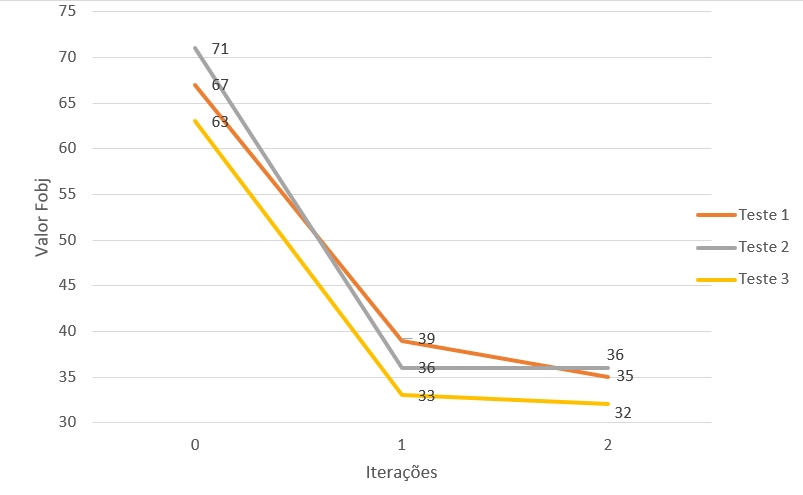
\includegraphics[scale=0.7]{figuras/VND_118_1_Aleat.jpg}
	\caption{Processo de Convergência rede 118 barras modificada teste 1 VNS-VND Aleatório.}
	\label{fig14} % mudar a referencia de acordo com o desejado
\end{figure}


\begin{figure}[H]
	\centering 
	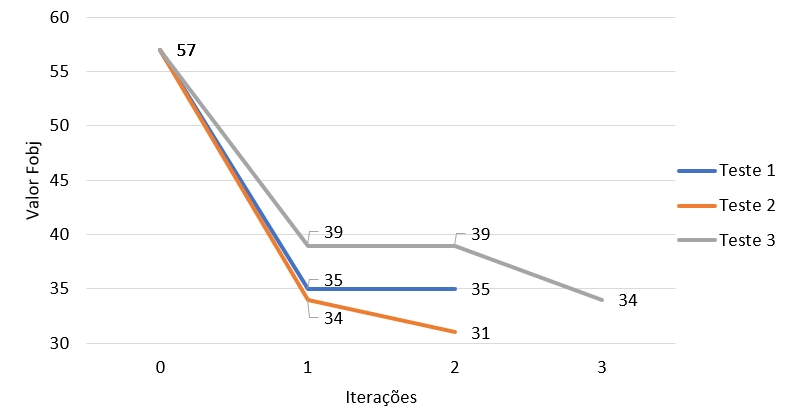
\includegraphics[scale=0.7]{figuras/VND_118_1_Guloso.jpg}
	\caption{Processo de Convergência rede 118 barras modificada teste 1 VNS-VND Guloso.}
	\label{fig15} % mudar a referencia de acordo com o desejado
\end{figure}


\begin{figure}[H]
	\centering 
	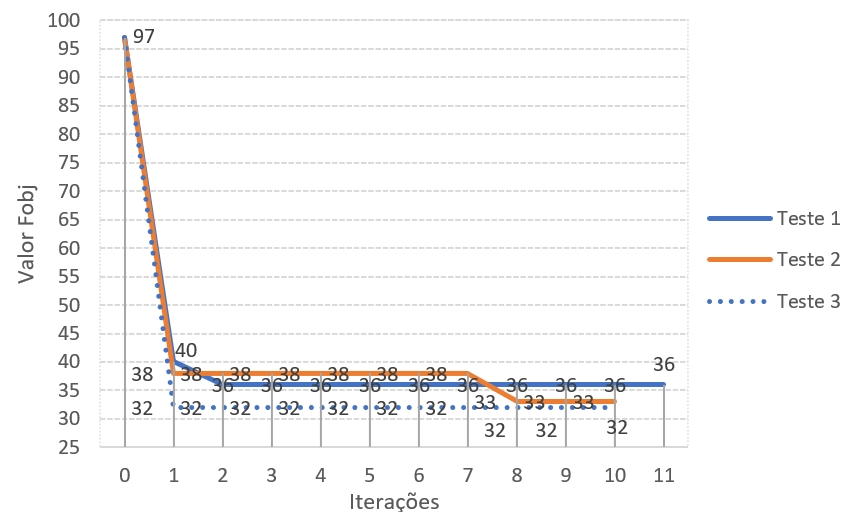
\includegraphics[scale=0.8]{figuras/GRASP_118_1_alpha03.jpg}
	\caption{Processo de Convergência rede 118 barras modificada teste 1 GRASP-VND $\alpha=0,3$.}
	\label{fig16} % mudar a referencia de acordo com o desejado
\end{figure}


\begin{figure}[H]
	\centering 
	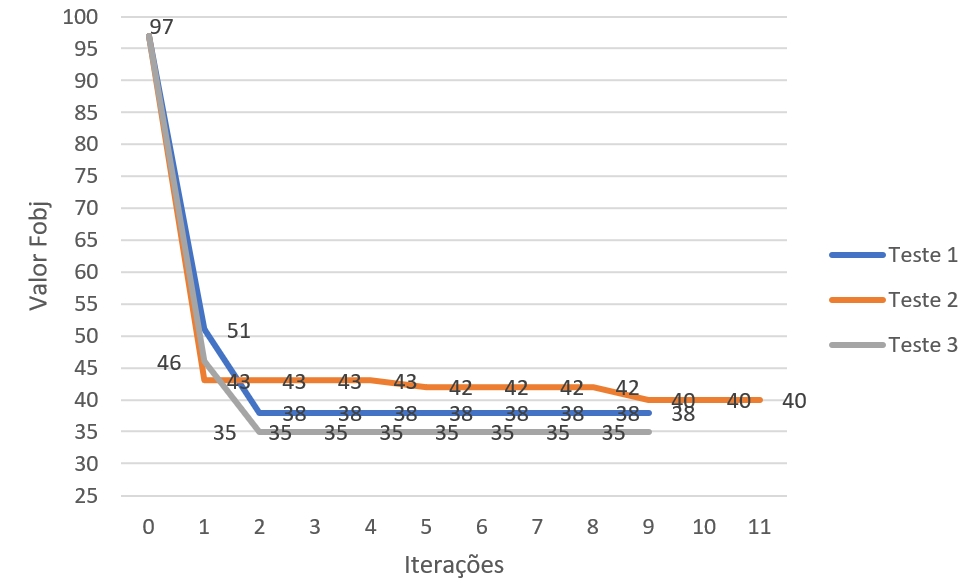
\includegraphics[scale=0.75]{figuras/GRASP_118_1_alpha08.jpg}
	\caption{Processo de Convergência rede 118 barras modificada teste 1 GRASP-VND $\alpha=0,8$.}
	\label{fig17} % mudar a referencia de acordo com o desejado
\end{figure}

Através dos resultados anteriores percebeu-se que as soluções iniciais com formação mais gulosa apresentaram melhores resultados que aquelas mais aleatórias. Isso indica que a estratégia de prioridades das barras é um bom caminho para se buscar melhores soluções para esse tipo de problema. Sendo assim as Tabelas abaixo se referem ao teste 2 realizado para a rede 118 barras modificada. Para tal configurou-se o algoritmo GRASP-VND com $\alpha=0.1$ e o VNS-VND com solução inicial gulosa. Além disso, para tentar realizar iterações mais rápidas utilizou-se apenas as duas primeiras estruturas de vizinhanças para a a etapa de busca local (VND). Para o VNS considerou-se, para a geração de vizinhos aleatórios, apenas as estruturas de vizinhança 1 e 2. Novamente estabeleceu-se como critério de parada dos testes um tempo máximo de 2h30min ou 20 iterações. Foram realizados 3 testes para cada uma das configurações e os resultados do processo de convergência seguem nos gráficos abaixo apresentados nas Figuras \ref{fig18} e \ref{fig19}. Todos os testes finalizaram com as 2h e 30 minutos de simulação e observa-se que neles não se conseguiu atingir o melhor resultado das simulações anteriores. Porém, a diminuição da quantidade de estruturas de vizinhança tornou a busca local mais rápida e permitiu uma maior quantidade de iterações, principalmente no algoritmo VNS-VND. O objetivo de promover mais iterações foi alcançado entretanto, em geral, ambas metaheurísticas estão convergindo para valores idênticos e ao atingi-los há uma dificuldade de melhoramento dessa solução. Na sequência dos estudos desse trabalho, visto que as metaheurísticas testadas se mostraram promissoras, o foco será em implementar estruturas mais sofisticadas e estratégias inteligentes para se atingir resultados melhores e mais estáveis para instâncias de maior complexidade.

\begin{figure}[H]
	\centering 
	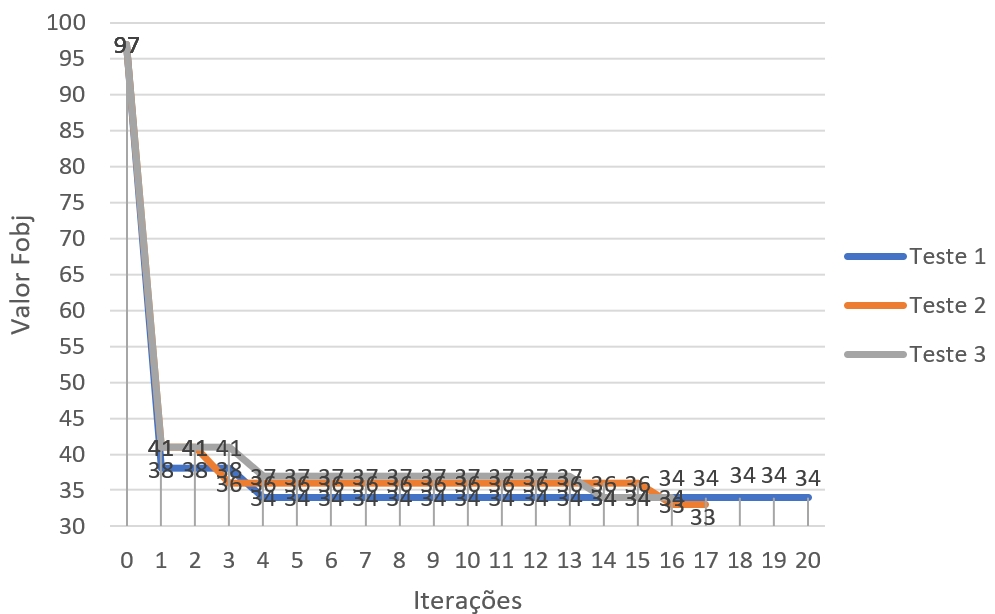
\includegraphics[scale=0.8]{figuras/GRASP_118_2_alpha01.jpg}
	\caption{Processo de Convergência rede 118 barras modificada teste 1 GRASP-VND $\alpha=0,1$.}
	\label{fig18} % mudar a referencia de acordo com o desejado
\end{figure}


\begin{figure}[H]
	\centering 
	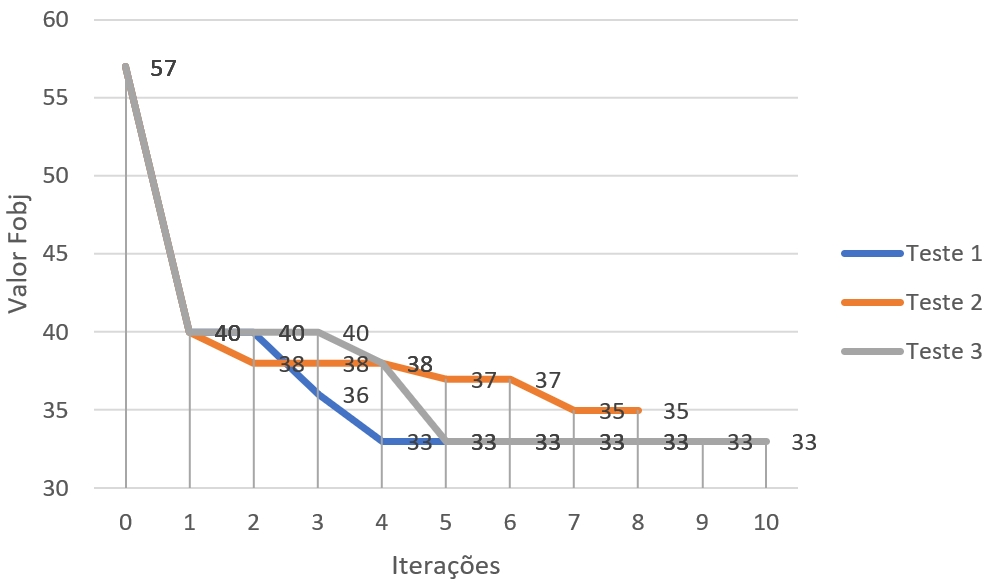
\includegraphics[scale=0.70]{figuras/VND_118_2_Guloso.jpg}
	\caption{Processo de Convergência rede 118 barras modificada teste 2 VNS-VND Guloso.}
	\label{fig19} % mudar a referencia de acordo com o desejado
\end{figure}


\section{Conclusões e Trabalhos Futuros}

O presente trabalho apresentou uma nova roupagem para o problema de alocação de UMs em redes elétricas. O objetivo de redução das criticalidades de medidas é ainda uma seara não explorada pelos pesquisadores, principalmente pela inexistência de uma técnica ou métrica estabelecida para avaliação dessas. Nesse trabalho conseguiu-se desenvolver uma formulação inicial para o problema considerando os pesos e as quantidades de criticalidades por cardinalidade. Essa função se apresentou promissora, mas há espaço para a inserção de restrições e fatores que insiram condições reais de operação, de maneira que ajudem, por exemplo, a diferenciar soluções em que as criticalidades são iguais. Apesar dessa função objetivo ser mais simples observou-se que foi possível reduzir com qualidade as criticalidades consideradas nos testes. Vale salientar que a possibilidade de inserir pesos proporciona uma flexibilidade em relação às prioridades desejadas.

Em relação às metaheurísticas testadas, ambas se mostraram promissoras e apresentaram resultados bons e equivalentes nos testes realizados. De fato, foi comprovado que uma busca exaustiva é impraticável para esse tipo de problema e as metaheurísticas são o caminho mais inteligente para se buscar boas soluções. Nos testes com a rede IEEE 30 barras tanto o GRASP-VND quanto o VNS-VND apresentaram desempenhos idênticos e conseguiram convergir para o valor ótimo, comprovado pela busca exaustiva completa. Nos testes com a rede 118 barras com a configuração base, novamente ambas metaheurísticas convergiram para valores iguais de função objetivo. Nessas instâncias mais complexas o custo para o cálculo das criticalidades passa a se apresentar como um fator que eleva o custo computacional do problema, o uso da tabela Hash Global atenuou parte desse custo, mas ainda há espaço para melhorias de desempenho. Como nesse trabalho não havia outras referências para se basear, o desempenho não foi o foco mas com esses resultados preliminares já é possível estabelecer comparações em trabalhos futuros.

Uma outra conclusão importante é a possibilidade de algumas configurações ligeiramente distintas resultarem em criticalidades iguais. Isso ocorre pois não é possível avaliar todas as criticalidades possíveis e nesse caso, para as condições avaliadas de fato as configurações se equivalem. Para trabalhos futuros a utilização de uma métrica em um pós-processamento, que consiga diferenciar essas configurações e escolher a melhor ou as melhores é um procedimento importante a ser realizado.

Por fim, criou-se uma instância deveras difícil e testou-se as metaheurísticas em duas condições distintas. Na primeira, considerou-se todas as estruturas de vizinhança criadas para a etapa de busca local, como resultado notou-se um elevado tempo despendido nessa etapa o que resultou em poucas iterações dentro do limite de tempo estabelecido. Apesar disso os algoritmos convergiram para valores de função objetivos próximos, mas o VNS-VND se destacou ao conseguir a melhor solução em um de seus testes, mostrando que o VNS e sua etapa de geração aleatória em uma vizinhança pode proporcionar fugas de mínimos locais. Na segunda condição, considerou-se soluções iniciais construídas de forma gulosa, além disso para se buscar mais iterações dentro do tempo limite, utilizou-se apenas as vizinhanças 1 e 2, na etapa de busca local. Como resultado confirmou-se que de fato, em ambos algoritmos, a busca local é a etapa mais densa e com essa redução realizou-se mais iterações, porém os resultados não superaram a melhor solução encontrada no teste anterior. Entretanto, quanto menos estruturas de vizinhança pode-se correr o risco de se estagnar em um dado valor de solução. Esse "\textit{trade-off}" deve ser mais bem avaliado e novas estruturas de vizinhança (mais sofisticadas) serem testadas.

Isto posto, o trabalho apresentou resultados promissores e indicou diversos caminhos interessantes para serem testados e avaliados em trabalhos futuros. Ambas metaheurísticas apresentaram bons resultados, com algumas vantagens para o GRASP-VND(iterações mais rápidas) e outras para o VNS-VND(resultados de qualidade com poucas iterações). Com esses pontos pode-se listar alguns testes e implementações a serem realizadas em trabalhos futuros:

\begin{itemize}
\item Testar uma busca local RVND para se tentar uma maior diversificação em instâncias maiores e complexas;
\item A utilização de um GRASP Reativo pode levar a um melhor conhecimento de qual $\alpha$ é mais interessante em cada instância testada;
\item Inserir conceitos de mineração de dados para a geração das soluções, visto que observou-se que as melhores apresentam diversos elementos em comum e isso pode ser uma característica própria de cada rede testada;
\item Inserção de restrições que indiquem prioridades em relações aos barramentos livres para alocação, considerando distâncias físicas e dificuldade de instalação por localidade;
\item Aprimoramento da função objetivo para considerar mais fatores além das criticalidades;
\item Desenvolvimento de outras funções para a etapa construtiva do GRASP, considerando não só uma informação heurística;
\item Geração de mais instâncias difíceis para testes e calibração das metaheurísticas;
\end{itemize}



\begin{thebibliography}{99}
	\bibitem{Abur04} Abur, A. Expósito, A. G. Power System State Estimation : Theory and Implementation. Marcel Dekker, New York, 2004.
	
	\bibitem{Mont99} Monticelli, A. State Estimation in Electric Power Systems: A Generalized Approach. Springer, New York, 1999.
	
	\bibitem{Marin03} F. J. Marin, F. Garcia-Lagos, G. Joya, and F. Sandoval, “Genetic algorithms for optimal placement of phasor measurement units in electric networks”, Electron. Lett. vol. 39, no. 19, pp. 1403-1405, Sep. 2003
	
	\bibitem{Aminifar09} F. Aminifar, C. Lucas, A. Khodaei, and M. Fotuhi-Firuzabad, “Optimal placement of phasor measurement units using immunity genetic algorithm”, IEEE Trans. Power Syst., vol. 24, no. 3, pp.1014-1020, July 2009. 
	
	\bibitem{Milosev03}  B. Milosevic and M. Begovic, “Nondominated sorting genetic algorithms for optimal phasor measurement placement”, IEEE Trans. Power Syst., vol. 18, no. 1, pp. 69-75, Feb. 2003. 
	
	\bibitem{PSO}  M. Hajain, A. M. Ranjbar, T. Amraee, and A. R. Shirani, “Optimal placement of phasor measurement units: Particle swarm optimization approach”, in Proc. Int. Conf. Intelligent Systems and Applications in Power Systems., pp. 1-6, Nov. 2007.
	
	\bibitem{BPSO} S. Chakrabarti, G.K. Venayagamoorthy, E. Kyriakides, PMU placement for power system observability using binary particle swarm optimization, in: Proceedings
	of Australasian Universities Power Engineering Conference, Sydney, Australia,
	December, 2008.
	
	\bibitem{SA} T. L. Baldwin, L. Mili, M. B. Boisen, Jr., and R. Adapa, “Power system observability with minimal phasor measurement placement”, IEEE Trans. Power Syst., vol. 8, no. 2, pp. 707-715, May 1993.
	
	\bibitem{TS} J. Peng, Y. Sun, and H. F. Wang, “Optimal PMU placement for full network observability using Tabu search algorithm”, Elec. Power Syst. Res., vol. 28, no. 4, pp. 223-231, May 2006. 
	
	\bibitem{Tree} R. F. Nuqui and A. G. Phadke, “Phasor measurement unit placement techniques for complete and incomplete observability”, IEEE Trans. Power Syst., vol. 20, no. 4, pp. 2381-2388, Oct. 2005.
	
	\bibitem{Abur04_opt} B. Xu and A. Abur, “Observability analysis and measurement placement for system with PMUs”, in Proc. IEEE Power System Conf. Expo., Oct. 2004, vol. 2, pp. 943-946.
	
	\bibitem{Amin10} F. Aminifar, A. Khodaei, M. Fotuhi-Firuzabad, and M. Shahidehpour, “Contingency-constrained PMU placement in power networks”, IEEE Trans. Power Syst., vol. 25, no. 1, pp. 516-523, Feb. 2010
	
	\bibitem{Gou08_1} B. Gou, “Generalized integer linear programming formulation for optimal PMU placement”, IEEE Trans. Power Syst., vol. 23, no. 3, pp. 1099-1104, Aug. 2008.
	
	\bibitem{Gou08_2} B. Gou, “Optimal placement of PMUs by integer linear programming”, IEEE Trans. Power Syst., vol. 23, no. 3, pp. 1525-1526, Aug. 2008.
	
	\bibitem{ReviewAlloc} W. Yuill, A. Edwards, S. Chowdhury and S. P. Chowdhury, "Optimal PMU placement: A comprehensive literature review," 2011 IEEE Power and Energy Society General Meeting, Detroit, MI, USA, 2011, pp. 1-8.
	
	\bibitem{AbelTese16} Augusto, A. A. Avaliação da Capacidade de Observação do Estado Operativo de Redes Elétricas. Tese de Doutorado, Instituto de Computação, Universidade Federal Fluminense, Niterói, RJ, Brasil, Fevereiro 2016.
	
	\bibitem{Sou12} K. C. Sou, H. Sandberg, and K. H. Johansson, “Computing critical ktuples in power networks,” IEEE Trans. Power Syst., vol. 27, no. 3, pp.
	1511-1520, Aug. 2012.
	
	\bibitem{BB16} Augusto, A. A.; Coutto Filho, M. B. D.; Souza, J. C. S.; Guimaraens, M.
	A. R. Branch-and-Bound Guided Search for Critical Elements in State Estimation.
	IEEE Trans. Power Syst. (2018).
	
	\bibitem{Hand07} Coutto Filho, M. B. D.; Souza., J. C. S. D.; Schilling, M. T. Handling
	Critical Data and Observability. Electric Power Components and Systems 35, 5
	(2007), 553-573.
	
	\bibitem{Mont85}A. Monticelli and F. F. Wu, “Network observability: Theory,” IEEE Trans. Power App. Syst., vol. PAS-104, no. 5, pp. 1035–1041, May 1985.
	
	\bibitem{AburObserv00} B. Gou and A. Abur, “A direct numerical method for observability analysis,” IEEE Trans. Power Syst., vol. 15, no. 2, pp. 625–630, May 2000.
	
	\bibitem{GRASP95}Feo, T.A.; Resende, M.G.C., Greedy randomized adaptive search procedures. Journal of Global Optimization 6, 109-133. (1995)

 	
	\bibitem{VND97}Mladenovic, N.; Hansen, P., Variable neighborhood Search. Computers and Operations Research, v. 24, 1097 – 1100. (1997)
	
	\bibitem{Quant13}M. B. Do Coutto Filho, J. C. Stacchini de Souza, and J. E. Villavicencio Tafur, “Quantifying observability in state estimation,” IEEE Trans. Power Syst., vol. 28, no. 3, pp. 2897-2906, Aug. 2013.
	
	\bibitem{Cormen}Cormen, T. H.; Leiserson, C. E.; Rivest, R. L.; Stein, C. Algoritmos, Teoria e Prática, 6 ed. Elsevier, Rio de Janeiro, 2002.

	
\end{thebibliography}


  

\end{document}
